\cleardoublepage\documentclass[../main.tex]{subfiles}
\begin{document}
\chapter{Derivadas}\index{Derivadas}\label{chap:derivadas}
\minitoc
%\tableofcontents
\subsection*{Objetivos de aprendizagem do capítulo}
\addcontentsline{toc}{section}{Objetivos de aprendizagem do capítulo}
Ao final deste capítulo você deverá ser capaz de:
\begin{itemize}
    \item Calcular a derivada de uma função como limite do quociente de incremento quando o incremento na variável independente tende a zero;
    \item   Interpretar geometricamente o conceito da derivada;
    \item Determinar a equação da reta tangente e normal em um ponto dado de uma curva;
    \item Aplicar os teoremas, para encontrar as derivadas de funções polinomiais e radicais;
    \item Calcular a derivada da composição de funções e a da inversa de uma função;
    \item Deduzir as fórmulas para encontrar as derivadas trigonométricas, logarítmicas, exponenciais e trigonométricas inversas;
    \item Derivar uma função dada implicitamente..
\end{itemize}
\section{Derivada no ponto}\index{Derivadas!no ponto}\label{sec:derivpt}

Nesta seção, vamos discutir sobre a noção de {\bf derivada de uma função em um ponto}. Começamos pelas noções de {\bf reta secante} e de {\bf reta tangente} ao gráfico de uma função. Em seguida, discutimos sobre as noções de {\bf taxa de variação média} e {\bf taxa de variação instantânea}. Por fim, definimos a derivada de uma função em um ponto.

\subsection{Reta secante e reta tangente}\index{Derivadas!reta tangente}
Definimos a {\bf reta secante} ao gráfico de uma dada função $f$ pelos pontos $x_0$ e $x_1$, $x_0\neq x_1$, como sendo a reta determinada pela equação
\begin{equation}
  y = \frac{f(x_1)-f(x_0)}{x_1-x_0}(x-x_0)+f(x_0)
\end{equation}
Isto é, é a reta que passa pelos pontos $(x_0,f(x_0))$ e $(x_1,f(x_1))$. Veja a Figura \ref{fig:retsectg}. Observemos que o coeficiente angular da reta secante é
\begin{equation}
  m_{\text{sec}} = \frac{f(x_1)-f(x_0)}{x_1-x_0}
\end{equation}
\begin{figure}[htb]
  \centering
  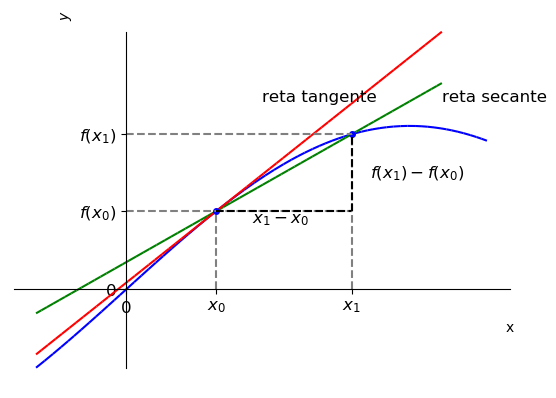
\includegraphics[width=0.7\textwidth]{fig_deriv/fig_retsectg}
  \caption{Esboços de uma reta secante (verde) e da reta tangente (vermelho) ao gráfico de uma função.}
  \label{fig:retsectg}
\end{figure}

A {\bf reta tangente} ao gráfico de uma função $f$ em $x=x_0$ é a reta que passa pelo ponto $(x_0, f(x_0))$ e tem coeficiente angular
\begin{equation}\label{eq:mtg}
  m_{\text{tg}} = \lim_{x_1\to x_0} \frac{f(x_1)-f(x_0)}{x_1-x_0}
\end{equation}
Isto é, a reta de equação
\begin{equation}
  \boldsymbol{y = m_{\text{tg}}(x-x_0)+f(x_0)}
\end{equation}
Menos formal, é a reta limite das retas secantes ao gráfico da função pelos pontos $x_0$ e $x_1$, quando $x_1\to x_0$. Veja a Figura \ref{fig:retsectg}.

\begin{obs}
  Fazendo $h = x_1-x_0$, temos que a Equação \ref{eq:mtg} é equivalente a
  \begin{equation}
    \boldsymbol{m_{\text{tg}} = \lim_{h\to 0} \frac{f(x_0+h)-f(x_0)}{h}}
  \end{equation}
\end{obs}

\begin{ex}
  Seja $f(x)=x^2$ e $x_0 = 1$. O coeficiente angular da reta secante ao gráfico de $f$ pelos pontos $x_0=1$ e $x_1 = 2$ é
  \begin{align*}
    m_{\text{sec}} &= \frac{f(x_1)-f(x_0)}{x_1-x_0}\\
                   &= \frac{f(2) - f(1)}{2-1}\\
                   &= 4-1 = 3
  \end{align*}
  Logo, a reta secante ao gráfico de $f$ pelos pontos $x_0=1$ e $x_1=2$ tem equação
  \begin{align*}
    y = m_{\text{sec}}(x-x_0) + f(x_0) &\Rightarrow y = 3(x-1)+f(1)\\
                                       &\Rightarrow y = 3x - 2
  \end{align*}
 Na Figura \ref{fig:cap_deriv_ex_rt_x2}, temos os esboços dos gráfico da função e da reta secante (verde).
  
  \begin{figure}[H]
    \centering
    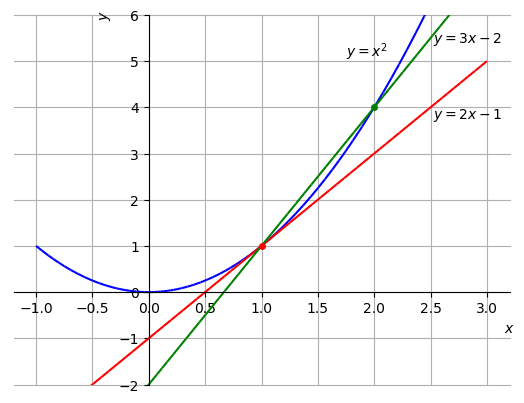
\includegraphics[width=0.7\textwidth]{fig_deriv/fig_cap_deriv_ex_rt_x2}
    \caption{Esboços dos gráficos de $f(x)=x^2$ (azul), da reta secante pelos pontos $x_0=1$ e $x_1=2$ (verde) e da reta tangente ao gráfico de $f$ no ponto $x_0 = 1$ (vermelho).}
    \label{fig:cap_deriv_ex_rt_x2}
  \end{figure}

  Agora, o coeficiente angular da reta tangente ao gráfico de $f$ no ponto $x_0$ é
  \begin{align*}
    m_{\text{tg}} &= \lim_{h\to 0} \frac{f(x_0+h)-f(x_0)}{h}\\
                  &= \lim_{h\to 0} \frac{(1+h)^2-1}{h}\\
                  &= \lim_{h\to 0} \frac{1+2h+h^2-1}{h}\\
                  &= \lim_{h\to 0} \frac{2+h}{1} = 2
  \end{align*}
  Assim sendo, a reta tangente ao gráfico de $f(x)=x^2$ no ponto $x_0=1$ tem coeficiente angular $m_{\text{tg}} = 2$ e equação
  \begin{equation*}
    y = 2(x-1)+1 = 2x-1
  \end{equation*}
  Na Figura \ref{fig:cap_deriv_ex_rt_x2}, temos os esboços dos gráfico da função e da reta tangente (vermelho).
  
  
  Com o \geogebra~ podemos obter a expressão da reta secante com os seguintes comandos:
\begin{verbatim}
x0 = 1
x1 = 2
f(x)= x^2
msec = (f(x1)-f(x0))/(x1-x0)
y=msec*(x-x0)+f(x0)
\end{verbatim}
A expressão da reta tangente pode ser obtida com os seguintes comandos:
\begin{verbatim}
x0 = 1
f(x)= x^2
mtg = limit((f(x0+x)-f(x0))/x,x,0)
y=mtg*(x-x0)+f(x0)
\end{verbatim}

\end{ex}

\subsection{Taxa de variação}
\begin{framed}
\begin{definition}
A {\bf taxa de variação média} de uma função $f$ quando $x$ varia de $x_0$ a $x_1$ é definida como
\begin{equation}
  \frac{\Delta y}{\Delta x} = \frac{f(x_1)-f(x_0)}{x_1-x_0}
\end{equation}
\end{definition}
\end{framed}

\begin{framed}
\begin{definition}
A {\bf taxa de variação instantânea} de $f$ no ponto $x_0$, a qual é definida como
\begin{align}
  \left.\frac{\dd f}{\dd x}\right|_{x=x_0} &= \lim_{x\to x_0} \frac{f(x)-f(x_0)}{x-x_0}\\
                             &= \lim_{h\to 0} \frac{f(x_0+h)-f(x_0)}{h}
\end{align}
onde $h=x-x_0\Rightarrow x=x_0+h$
\end{definition}\end{framed}
Em muitas áreas do conhecimento, estas taxa recebem nomes específicos.

\begin{ex}
  Seja $s = s(t)$ a função distância percorrida por um objeto no tempo. A {\bf velocidade média} (taxa de variação média da distância) do tempo $t_0$ ao tempo $t_1$ é
  \begin{equation*}
    \frac{\Delta s}{\Delta t} = \frac{s(t_1)-s(t_0)}{t_1-t_0}
  \end{equation*}
  Por exemplo, se $s(t) = 15t^2+t$ (km), então a velocidade média do objeto entre $t_0=1$h e $t_1=3$h é
  \begin{align*}
    \frac{\Delta s}{\Delta t} &= \frac{(15t_1^2+t_1)-(15t_0^2+t_0)}{t_1-t_0}\\
                              &= \frac{15\cdot 3^2+3-(15\cdot 1^2+1)}{3-1}\\
                              &= \frac{135+3-15-1}{2}\\
                              &= 61~\frac{\text{km}}{\text{h}}
  \end{align*}

  A {\bf velocidade} (taxa de variação instantânea da distância) no tempo $t_0=1$ é
  \begin{align*}
    \left.\frac{\dd s}{\dd t}\right|_{t=t_0} &= \lim_{h\to 0} \frac{s(t_0+h)-s(t_0)}{h} \\
                                             &= \lim_{h\to 0} \frac{15(t_0+h)^2+(t_0+h)-\left(15t_0^2+t_0\right)}{h}\\
                                             &= \lim_{h\to 0} \frac{15t_0^2+30t_0h+15h^2+t_0+h-15t_0^2-t_0}{h}\\
                                             &= \lim_{h\to 0} \frac{30t_0h+15h^2+h}{h}\\
                                             &= \lim_{h\to 0} 30t_0 + 15h + 1= 30t_0+1 = 31~\frac{\text{km}}{\text{h}}
  \end{align*}
\end{ex}

\begin{ex}
  Seja $c(x) = \sqrt{x}$ (milhões de reais) o custo da produção em uma empresa em função do número de unidades produzidas (milhares). O {\bf custo médio da produção} de $x_0=4$ a $x_1=9$ é
  \begin{align*}
    \frac{\Delta c}{\Delta x} &= \frac{c(x_1)-c(x_0)}{x_1-x_0}\\
                              &= \frac{\sqrt{x_1}-\sqrt{x_0}}{x_1-x_0}\\
                              &= \frac{\sqrt{9}-\sqrt{4}}{9-4}\\
                              &= \frac{3-2}{5}= 0,2~\frac{\text{R\$}}{\text{un}}
  \end{align*}

  O {\bf custo marginal} (taxa de variação instantânea do custo) quando a empresa está produzindo $x_0=4$ milhões de unidades é
  \begin{align*}
    \left.\frac{\dd c}{\dd x}\right|_{x=x_0=4} &= \lim_{h\to 0} \frac{\sqrt{x_0+h}-\sqrt{x_0}}{h}\\
                                               &= \lim_{h\to 0} \frac{\sqrt{x_0+h}-\sqrt{x_0}}{h}\cdot \frac{\sqrt{x_0+h}+\sqrt{x_0}}{\sqrt{x_0+h}+\sqrt{x_0}}\\
                                               &= \lim_{h\to 0} \frac{x_0+h-x_0}{h(\sqrt{x_0+h}+\sqrt{x_0})}\\
                                               &= \lim_{h\to 0} \frac{1}{\sqrt{x_0+\cancelto{0}{h}}+\sqrt{x_0}}\\
                                               &= \frac{1}{2\sqrt{x_0}} = \frac{\sqrt{x_0}}{2x_0}\\
                                               &= \frac{\sqrt{4}}{2\cdot 4} = 0,25~\frac{\text{R\$}}{\text{un}}
  \end{align*}
\end{ex}

\begin{obs}
  Analogamente a custo marginal, temos as noções de rendimento marginal e lucro marginal.
\end{obs}

\subsection{Derivada em um ponto}

A {\bf derivada} de uma função $f$ {\bf em um ponto} $x=x_0$ é denotada por $f'(x_0)$ ou $\displaystyle \frac{\dd f}{\dd x}(x_0)$ e é definida por
\begin{equation}
  f'(x_0) = \left.\frac{\dd f}{\dd x}\right|_{x=x_0} = \lim_{h\to 0} \frac{f(x_0+h)-f(x_0)}{h}.
\end{equation}

\begin{ex}
  Vejamos os seguintes casos:
  \begin{enumerate}[a)]
  \item $f(x) = k$, $k$ constante.
    \begin{align*}
      f'(x_0) &= \lim_{h\to 0} \frac{f(x_0+h)-f(x_0)}{h}\\
              &= \lim_{h\to 0} \frac{k-k}{h} = 0.
    \end{align*}
  \item $f(x) = x$.
    \begin{align*}
      f'(x_0) &= \lim_{h\to 0} \frac{f(x_0+h)-f(x_0)}{h} \\
              &= \lim_{h\to 0} \frac{x_0+h-x_0}{h} = 1
    \end{align*}
  \item $f(x) = \sqrt{x}$, $x_0=1$.
    \begin{align*}
      f'(1) &= \lim_{h\to 0} \frac{\sqrt{1+h}-\sqrt{1}}{h}\\
            &= \lim_{h\to 0} \frac{\sqrt{1+h}-\sqrt{1}}{h} \cdot \frac{\sqrt{1+h}+\sqrt{1}}{\sqrt{1+h}+\sqrt{1}}\\
            &= \lim_{h\to 0} \frac{1+h-1}{h(\sqrt{1+h}+1)} = \frac{1}{2}
    \end{align*}
  \end{enumerate}
\end{ex}

\begin{ex}
  Assuma que o rendimento de uma empresa é modelado por $r(x) = x^2$ (milhões de reais), onde $x$ é o número em milhões de unidades vendidas. O {\bf rendimento marginal} quando $x=x_0=1$ é
  \begin{align*}
    r'(x_0) &= \lim_{x\to x_0}\frac{(x_0+h)^2-x_0^2}{h}\\
            &= \lim_{x\to x_0}\frac{x_0^2+2x_0h+h^2-x_0^2}{h}\\
            &= \lim_{x\to x_0} 2x_0h + h = 2x_0 = 2~\frac{\text{R\$}}{\text{un}}
  \end{align*}
\end{ex}

\subsection{Exercícios resolvidos}

\begin{exeresol}
  Determine a equação da reta tangente ao gráfico de $f(x) = \sqrt{x}$ no ponto $x_0=4$. Faça, então, os esboços dos gráficos de $f$ e da reta tangente em um mesmo plano cartesiano.
\end{exeresol}
\begin{resol}
  A equação da reta tangente ao gráfico da função $f$ no ponto $x_0=4$ é
  \begin{equation}
    y = f'(x_0)(x-x_0)+f(x_0).
  \end{equation}
  A derivada de $f$ no ponto $x_0$ é
  \begin{align*}
    f'(x_0) &= \lim_{x\to x_0} \frac{f(x_0+h)-f(x_0)}{h}\\
            &= \lim_{x\to 4} \frac{\sqrt{4+h}-\sqrt{4}}{h}\\
            &= \lim_{x\to 4} \frac{\sqrt{4+h}-2}{h} \cdot \frac{\sqrt{4+h}+2}{\sqrt{4+h}+2}\\
            &= \lim_{x\to 4} \frac{4+h-4}{h(\sqrt{4+h}+2)}\\
            &= \frac{1}{\sqrt{4}+2} = \frac{1}{4}.
  \end{align*}
  Portanto, a equação da reta tangente é
  \begin{equation*}
    y = \frac{1}{4}(x-4)+\sqrt{4} \Rightarrow y = \frac{1}{4}x+1
  \end{equation*}
  Veja a Figura \ref{fig:cap_deriv_exeresol_rt_sqrt} para os esboços dos gráfico de $f$ e da reta tangente.

  \begin{figure}[H]
    \centering
    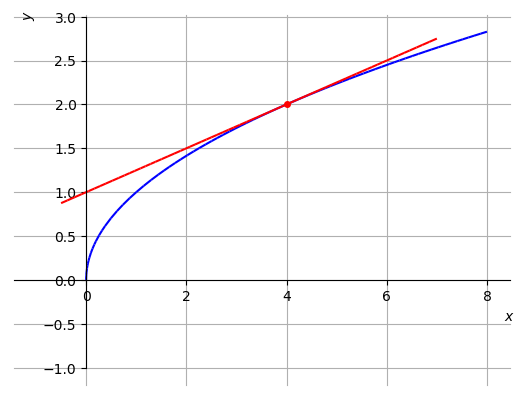
\includegraphics[width=0.7\textwidth]{fig_deriv/fig_cap_deriv_exeresol_rt_sqrt}
    \caption{Esboços do gráfico da função $f$ e da reta tangente no ponto $x_0=4$.}
    \label{fig:cap_deriv_exeresol_rt_sqrt}
  \end{figure}
\end{resol}

\begin{exeresol}
  Considere que a produção em uma empresa tem custo
  \begin{equation*}
    c(x) = \sqrt{x}
  \end{equation*}
  e rendimento
  \begin{equation*}
    r(x) = x^1
  \end{equation*}
  onde $x$ é o número de unidades (em milhões) produzidas. Calcule o lucro marginal da empresa quando $x=1$ mi.
\end{exeresol}
\begin{resol}
  O lucro é
  \begin{equation*}
    l(x) = r(x) - c(x).
  \end{equation*}
  Desta forma, o lucro marginal no ponto $x_0=1$ é
  \begin{align*}
    l'(x_0) &= \lim_{h\to 0} \frac{l(x_0+h)-l(x_0)}{h}\\
            &= \lim_{h\to 0} \frac{r(x_0+h)-c(x_0+h)-(r(x_0)-c(x_0))}{h}\\
            &= \lim_{h\to 0} \frac{r(x_0+h)-r(x_0) - (c(x_0+h)-c(x_0))}{h}\\
            &= \lim_{h\to 0} \frac{r(x_0+h)-r(x_0)}{h} - \lim_{h\to 0} \frac{c(x_0+h)-c(x_0)}{h}\\
            &= r'(x_0) - c'(x_0)\\
            &= 2x_0 - \frac{1}{2\sqrt{x_0}}\\
            &= 2 - \frac{1}{2} = 1,5~\frac{\text{R\$}}{\text{un}}.
  \end{align*}
\end{resol}


\subsection{Exercícios}
\begin{exer}
  Encontre a equação da reta tangente à curva $y= f(x)$ no ponto $P$:
   \begin{enumerate}[a)]
  \item  $f(x)=\frac{1}{x}; P=\pc{\frac{1}{2},2}$
  \item  $f(x)=2x^2+x+2; P=\pc{-1,3}$
  \end{enumerate}
\end{exer}
\begin{resp}
 a) $y = -4x + 4$\hspace{2cm} b) $y = -3x - 2$
\end{resp}
\begin{exer}
  Calcule as derivadas conforme indicado:
  \begin{enumerate}[a)]
  \item $f(x) = 2$, $f'(-1)$
  \item $g(x) = 10^6$, $g'(10^8)$
  \item $h(x) = \ln 2e$, $h'(-\pi)$
  \end{enumerate}
\end{exer}
\begin{resp}
  a)~$0$; b)~$0$; c)~$0$
\end{resp}

\begin{exer}
  Calcule as derivadas conforme indicado:
  \begin{enumerate}[a)]
  \item $f(x) = 2 + x$, $f'(-1)$
  \item $g(x) = 10^6 - 2x$, $g'(-3)$
  \item $h(x) = \ln(2e) + ex$, $h'(10^6)$
  \end{enumerate}  
\end{exer}
\begin{resp}
  a)~$-1$; b)~$-2$; c)~$e$
\end{resp}

\begin{exer}
  Calcule as derivadas conforme indicado:
  \begin{enumerate}[a)]
  \item $f(x) = x$, $f'(-1)$
  \item $g(x) = -2x$, $g'(-3)$
  \item $h(x) = ex$, $h'(10^6)$
  \end{enumerate}  
\end{exer}
\begin{resp}
  a)~$-1$; b)~$-2$; c)~$e$
\end{resp}

\begin{exer}
  Determine a reta secante ao gráfico de $f(x) = 5-x^2$ pelos pontos $x_0=1$ e $x_1=2$. Então, determine a reta tangente ao gráfico de $f$ no ponto $x_0=1$. Por fim, faça os esboços dos gráficos de $f$, da reta secante e da reta tangente em um mesmo plano cartesiano.
\end{exer}
\begin{resp}
  reta secante: $y = -3x + 7$; reta tangente: $y = -2x + 6$; dica: verifique seus esboços plotando os gráficos no computador
\end{resp}

\begin{exer}
  Assumindo que, em uma empresa, a produção tenha o custo $c(x) = 2\sqrt{x}$ e rendimento $r(x) = \frac{1}{100}x^3$, dados em milhões de reais com $x$ em milhares de unidades. Calcule:
  \begin{enumerate}[a)]
  \item o custo marginal quando $x = 1$
  \item o rendimento marginal quando $x = 1$
  \item o lucro marginal quando $x=1$
  \end{enumerate}
\end{exer}
\begin{resp}
  a)~$1000~\frac{\text{R}\$}{\text{un}}$; b)~$30~\frac{\text{R\$}}{\text{un}}$; c)~$-970~\frac{\text{R\$}}{\text{un}}$
\end{resp}

\section{Função derivada}\label{cap_deriv_sec_funder}
\begin{framed}
\begin{definition}
A {\bf derivada} de uma função $f$ em relação à variável $x$ é a função $\displaystyle f' = \frac{\dd f}{\dd x}$ cujo valor em $x$ é
\begin{equation}\label{eq:derivada}
  f'(x) = \lim_{h\to 0} \frac{f(x+h)-f(x)}{h}
\end{equation}
quando este limite existe. Dizemos que $f$ é {\bf derivável} (ou {\bf diferenciável}) em um ponto $x$ de seu domínio, quando o limite dado em \ref{eq:derivada} existe. Se isso ocorre para todo número real $x$, dizemos que $f$ é derivável em toda parte.
\end{definition}
\end{framed}

\begin{ex}
  A derivada de $f(x) = x^2$ é
  \begin{align*}
    f'(x) &= \lim_{h\to 0} \frac{f(x+h)-f(x)}{h}\\
          &= \lim_{h\to 0} \frac{(x+h)^2 - x^2}{h}\\
          &= \lim_{h\to 0} \frac{x^2+2xh+h^2-x^2}{h}\\
          &= \lim_{h\to 0} 2x+h = 2x
  \end{align*}
  Observamos que este é o caso de uma função derivável em toda parte. A Figura \ref{fig:deriv_ex_ffl_x2}. esboça o gráfico da função $f(x)=x^2$ e de sua derivada.

  \begin{figure}[H]
    \centering
    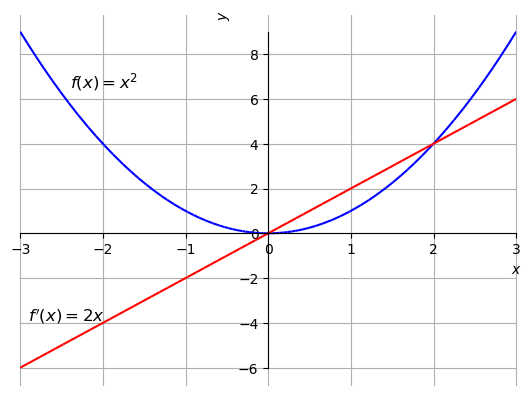
\includegraphics[width=0.65\textwidth]{fig_deriv/fig_deriv_ex_ffl_x2}
    \caption{Esboços dos gráficos da função $f(x)=x^2$ e de sua derivada $f'(x) = 2x$.}
    \label{fig:deriv_ex_ffl_x2}
  \end{figure}  
  No \geogebra, podemos fazer este cálculo com o comando \verb+derivada(f)+, após ter definida $f$ como \verb+f(x)=x^2+
 \end{ex}
 \section{Derivadas Laterais}\hypertarget{DerivLaterais}{}\label{sec:DerivLaterais}
 Desde que a derivada é um limite, é importante saber o que acontece quando nos aproximamos por meio de valores menores e maiores do ponto analisado, na expressão da derivada.
 \begin{framed}
 \begin{definition}
 Seja \(f: \mathbb{R} \to \mathbb{R}\) uma função e \(x_0\in {\rm Dom}(f)\).
 \begin{compactenum}[i. ]
\item A derivada pela esquerda de \(f\) no ponto \(x_0\), denotada por \(f'_-(x_0)\), é definida por

\[ f'_-(x_0)=\lim\limits_{h\rightarrow 0^-} \dfrac{f(x_0+h)-f(x_0)}{h} \]
se este limite existe.

\item A derivada pela direita de \(f\) no ponto \(x_0\), denotada por \(f'_+(x_0)\), é definida por

\[ f'_+(x_0)=\lim\limits_{h\rightarrow 0^+} \dfrac{f(x_0+h)-f(x_0)}{h} \]
se este limite existe.
\end{compactenum}
 \end{definition}
 \end{framed}
 \begin{framed}
\begin{prop}
Seja $f$ uma função definida em $(a,b)$, com $x_0\in (a,b)$. A derivada de $f$ em $x_0$ existe se, e somente se, as derivadas laterais $f'_{-}(x_0)$ e $f'_{-}(x_0)$ existem e são iguais.
\end{prop}
\end{framed}
 \begin{ex}\label{ex:Deriv-FuncValorAbs}
  A função valor absoluto é derivável para todo $x\neq 0$ e não é derivável em $x=0$. De fato, para $x<0$ temos
  \begin{align*}
    f'(x) &= \lim_{h\to 0} \frac{|x+h|-|x|}{h}\\
          &= \lim_{h\to 0} \frac{-(x+h)+x}{h}\\
          &= \lim_{h\to 0} \frac{-h}{h} = -1
  \end{align*}
  Analogamente, para $x>0$ temos
  \begin{align*}
    f'(x) &= \lim_{h\to 0} \frac{|x+h|-|x|}{h}\\
          &= \lim_{h\to 0} \frac{x+h-x}{h}\\
          &= \lim_{h\to 0} \frac{h}{h} = 1
  \end{align*}
  Agora, para $x=0$, devemos verificar as derivadas laterais:
  \begin{align*}
    f'_+(0) &= \lim_{h\to 0^+} \frac{|h|-|0|}{h} = \lim_{h\to 0^+} \frac{h}{h} = 1\\
    f'_-(0) &= \lim_{h\to 0^-} \frac{|h|-|0|}{h} = \lim_{h\to 0^-} \frac{-h}{h} = -1
  \end{align*}
  Como as derivadas laterais são diferentes, temos que $y = |x|$ não é derivável em $x=0$. Na figura \ref{fig:deriv_ex_ffl_absx}, temos os esboços dos gráficos de $f(x) = |x|$ e sua derivada
  \begin{equation}\label{eq:deriv_signx}
    f'(x) = \left\{
      \begin{array}[H]{rr}
        -1, & x<0\\
        1, & x> 0
      \end{array}
    \right.
  \end{equation}
  Esta é chamada de {\bf função sinal} e denotada por $\sign(x)$. Ou seja, a função sinal é a derivada da função valor absoluto.

  \begin{figure}[H]
    \centering
    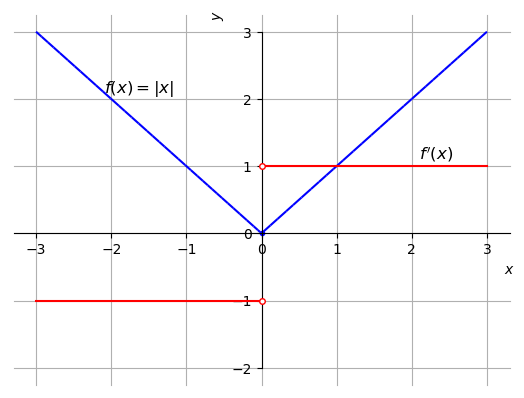
\includegraphics[width=0.7\textwidth]{fig_deriv/fig_deriv_ex_ffl_absx}
    \caption{Esboços dos gráficos da função $f(x)=|x|$ e de sua derivada.}
    \label{fig:deriv_ex_ffl_absx}
  \end{figure}
\end{ex}
\begin{ex}\label{ex:deriv_sqrtx}
  Vamos calcular a derivada de $f(x) = \sqrt{x}$. Para $x=0$. Neste caso só faz sentido calcular a derivada lateral à direta:
  \begin{align*}
    f'_{+}(0) &= \lim_{h\to 0^+} \frac{\sqrt{0+h}-\sqrt{0}}{h} \\
              &= \lim_{h\to 0^+} \frac{\sqrt{h}}{h} \\
              &= \lim_{h\to 0^+} \frac{1}{\cancelto{0^+}{\sqrt{h}}} = +\infty
  \end{align*}
  Ou seja, $f(x) = \sqrt{x}$ não é derivável em $x=0$. Agora, para $x> 0$, temos
  \begin{align}
    f'(x) &= \lim_{h\to 0} \frac{\sqrt{x+h}-\sqrt{x}}{h}\nonumber\\
          &= \lim_{h\to 0} \frac{\sqrt{x+h}-\sqrt{x}}{h}\cdot \frac{\sqrt{x+h}+\sqrt{x}}{\sqrt{x+h}+\sqrt{x}}\nonumber\\
          &= \lim_{h\to 0} \frac{x+h-x}{h(\sqrt{x+h}+\sqrt{x})}\nonumber\\
          &= \frac{1}{2\sqrt{x}}\label{eq:DerivRaizX}
  \end{align}
  Na Figura \ref{fig:deriv_ex_ffl_sqrtx}, temos os esboços dos gráficos desta função e de sua derivada.

  \begin{figure}[H]
    \centering
    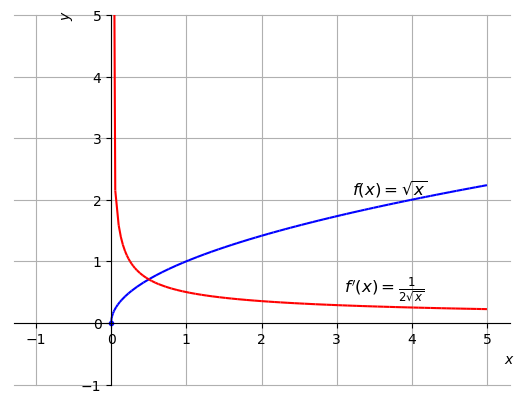
\includegraphics[width=0.65\textwidth]{fig_deriv/fig_deriv_ex_ffl_sqrtx}
    \caption{Esboços dos gráficos da função $f(x)=\sqrt{x}$ e de sua derivada.}
    \label{fig:deriv_ex_ffl_sqrtx}
  \end{figure}
\end{ex}

O próximo resultado mostra que funções não são diferenciáveis em pontos de descontinuidade
\begin{framed}
\begin{prop}\label{prop:FDeriv-Dif}
Se a função \(f: \mathbb{R} \to \mathbb{R}\) é derivável no ponto \(a\in {\rm Dom}(f)\), então \(f\) é contínua no ponto \(a\).
\end{prop}
\end{framed}
\nota{
A recíproca da Proposição \ref{prop:FDeriv-Dif} não é necessariamente verdadeira. Se consideramos a função \(f(x)=|x|\), sabemos que ela é contínua em \(x=0\). Porém, conforme será mostrado no Exemplo \ref{ex:Deriv-FuncValorAbs}, ela não é derivável em \(x=0\).

Para encontrar as derivadas laterais das funções definidas por partes nos pontos onde a função muda de regra de correspondência é útil ter em mente as seguintes propriedades:

Se \(f\) é derivável para todo \(x<x_0\), \(\lim\limits_{x\rightarrow x_0^-}f(x)=f(x_0)\) e \(\lim\limits_{x\rightarrow x_0^-}f'(x)=L\) existe, então,

\[ f'_-(x_0)=L. \]
Se \(f\) é derivável para todo \(x>x_0\), \(\lim\limits_{x\rightarrow x_0^+}f(x)=f(x_0)\) e \(\lim\limits_{x\rightarrow x_0^+}f'(x)=L\) existe, então,

\[ f'_+(x_0)=L. \]
}

\desafio{\hypertarget{desafio}{Considerando a aproximação} $$f'(x)\approx \frac{f(x+\Delta x)-f(x)}{\Delta x}\Rightarrow f(x+\Delta x)\approx f(x)+f'(x)\Delta x$$ e a derivada da função $f(x)=\sqrt{x}$ \eqref{eq:DerivRaizX}, obtida no exemplo anterior. Encontre uma fórmula para o cálculo de raízes aproximadas de funções quadráticas, utilizando derivada. Aplique-a para alguns exemplos de sua escolha.
}
\vspace{0.3cm}
\begin{ex}
  Seja a função \(f\) definida por:

\[ f(x)=\left\{ \begin{array}{ccl} x^2, & &\mbox{ se }\, x<1;\\ ax+b, & &\mbox{ se }\, x\geq 1. \end{array} \right. \]
Determinemos os valores de \(a\) e \(b\) para que \(f'(1)\) exista.

\begin{solut}
Considerando que \(f'(1)\) existe, então \(f\) é contínua no ponto \(x=1\). Logo, obtemos \(\lim\limits_{x\rightarrow 1^-}f(x)=\lim\limits_{x\rightarrow 1^+}f(x)\) e, assim, obtemos que \(1=a+b\).
Por outro lado,

\[ f'(x)=\left\{ \begin{array}{ccl} 2x, & &\mbox{ se }\, x<1;\\ a, & &\mbox{ se }\, x> 1. \end{array} \right. \]
Pela nota anterior, temos que

\[ f'(1^-)=\lim\limits_{x\rightarrow 1^-}f(x)=2 \quad \mbox{e}\quad f'(1^+)=\lim\limits_{x\rightarrow 1^+}f(x)=a, \]
e como \(f'(1)\) existe, resulta \(a=2\). Finalmente, da condição \(a+b=1\) obtemos que \(b=-1\).


\end{solut}
\end{ex}
\begin{ex}
  Determinemos se a função \(f\) definida por:

\[ f(x)=\left\{ \begin{array}{ccl} x, & &\mbox{ se }\, x\leq 0;\\ x^2, & &\mbox{ se }\, x> 0; \end{array} \right. \]
é derivável no ponto \(x=0\).

\begin{solut}
Da definição de \(f\), temos que

\[ \begin{array}{l} f'(0^-)= \lim\limits_{h\rightarrow 0^-}\dfrac{f(0+h)-f(0)}{h}=\lim\limits_{x\rightarrow h^-}\dfrac{h}{h}=1,\\ f'(0^+)= \lim\limits_{h\rightarrow 0^+}\dfrac{f(0+h)-f(0)}{h}=\lim\limits_{x\rightarrow h^+}\dfrac{h^2}{h}=\lim\limits_{h\rightarrow 0^+}h=0. \end{array} \]
Portanto, a função não é derivável no ponto \(x=0\), porém, é contínua no ponto \(x=0\).
\end{solut}
\end{ex}
\section{Reta Normal}
Ao considerar a interpretação geométrica da derivada em um ponto, entendemos como a equação da reta tangente, denotada por \(L_T\) é obtida. Agora vamos a analisar a reta perpendicular a esta.
\begin{framed}
\begin{definition}
Seja \(f: \mathbb{R} \to \mathbb{R}\) uma função derivável no ponto \(x=x_0\). A reta que passa pelo ponto \((x_0,f(x_0))\) e é perpendicular à reta tangente da curva \(y=f(x)\) no ponto \((x_0,f(x_0))\) é chamada de reta normal da curva \(y=f(x)\) no ponto \((x_0,f(x_0))\), denotada por \(L_N\), e se:

\(f'(x_0)\neq 0\), então a equação da reta normal é

\[ L_N\,:\quad y-f(x_0)=-\dfrac{1}{f'(x_0)}(x-x_0); \]
\(f'(x_0)= 0\), então a equação da reta normal é

\[ L_N\,:\quad x-x_0=0. \]
\end{definition}
\end{framed}
\begin{figure}[htb]
    \centering
    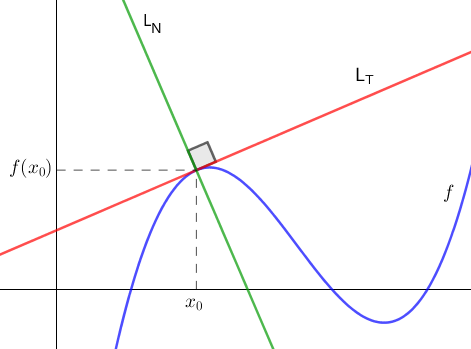
\includegraphics[scale=0.7]{3-cap_derivadas/fig_deriv/RetaTangente-Normal.png}
    \caption{Representação da reta normal a uma função no ponto $(x_0,f(x_0))$}
    \label{fig:RetaTangNormal}
\end{figure}
\begin{ex}
  Seja \(f(x)=x^2-2x+3\), encontremos as equações da reta tangente \(L_T\) e da reta normal \(L_N\) à curva \(y=f(x)\) no ponto \((2,3)\).
  
  \begin{solution}
  Desde que as equações de \(L_T\) e \(L_N\) no ponto \((2,3)\) dependem de \(f'(2)\), calculemos este valor

\[ f'(2)=\lim\limits_{h\rightarrow 0}\dfrac{f(2+h)-f(2)}{h}=\lim\limits_{h\rightarrow 0}(h+2)= 2. \]
Assim, as equações das retas tangente e normal à curva \(y=f(x)\) no ponto \((2,3)\) são:

\[ \begin{array}{l} L_T\,:\,y-3=2(x-2)\,\Leftrightarrow\,\boldsymbol{L_T\,:\,2x-y-1=0}\\ L_N\,:\,y-3=-\dfrac{1}{2}(x-2)\,\Leftrightarrow\,\boldsymbol{L_N\,:\,x+2y-8=0}. \end{array} \]
  \end{solution}
\end{ex}
\begin{ex}
  Determinemos \((a,f(a))\) e as equações das retas tangente e normal à curva \(y=f(x)=2-x-x^2\), sendo que a reta tangente é paralela à reta \( x-y-4=0\).
  
  \begin{solution}
O nosso problema aqui é encontrar o ponto \((a,f(a))\) no qual a reta esta definida. Porém, a reta paralela \( x-y-4=0\) nos dará essa informação.

Calculando a derivada

\[ f'(a)=\lim\limits_{h\rightarrow 0}\dfrac{f(a+h)-f(a)}{h}=\lim\limits_{h\rightarrow 0}(-1-2a-h)= -1-2a. \]
Como as inclinações de \( x-y-4=0\) e \(L_T\) são iguais, então \(f'(a) =1\). Logo, destas duas equações, obtemos que \(a=-1\). Portanto, o ponto de tangência é \((-1,f(-1))=(-1,2)\), e as equações das retas tangente e normal são:

\[ L_T: \quad y=x+3\quad \mbox{e}\quad L_N: \quad y=-x+1, \]
respectivamente.\\
\dica \textit{Ocultamos alguns passos, como os cálculos relativos a encontrar as equações das retas tangente e normal.}
  \end{solution}
\end{ex}
\begin{ex}
  Dada a reta \(L_N\), normal à curva \(y=f(x)=x^2-4\) no ponto \((a,f(a))\). Se \(L_N\) passa pelo ponto \((33,0)\), determinemos o valor de \(a\) e as equações de \(L_T\) e \(L_N\).

\begin{solution}
Como \(f'(x)=2x\), a inclinação de \( L_{T}\) no ponto \((a,f(a))\) é \( f'(a)=2a\). Por outro lado, a inclinação da reta \(L_N\) que passa pelos pontos \((33,0)\) e \((a,f(a))\) é

\[ -\dfrac{1}{f'(a)}= \dfrac{f(a)-0}{a-33}=\dfrac{a^2-4}{a-33} \]
Logo,

\[ 2a^3-7a-33=0\quad\Rightarrow\quad (a-3)(2a^2+6a+11)=0. \]
Em consequência, \(a=3\), pois é a única raiz real da equação acima, e as equações das retas tangente e normal são:

\[ L_T: \quad y=6x-13\quad \mbox{e}\quad L_N: \quad y=-\dfrac{1}{6}x+\dfrac{11}{2}, \]
respectivamente.
\end{solution}

\end{ex}
\hypertarget{DerivOrdemSup}{\section{Derivadas de ordem superior}}\index{Derivadas!Ordem Superior}\label{sec:DerivOrdemSuperior}

A derivada de uma função $y = f(x)$ em relação a $x$ é a função $y = f'(x)$. Quando esta é diferenciável, podemos calcular a derivada da derivada. Esta é conhecida como a {\bf segunda derivada} de $f$, denotamos
\begin{equation}
  f''(x) = (f'(x))' ~\quad \text{ou} ~\quad \frac{\dd^2}{\dd x^2}f(x) = \frac{\dd}{\dd x}\left(\frac{\dd}{\dd x}f(x)\right).
\end{equation}

\begin{ex}\label{ex:deriv_fll}
  Seja $f(x) = x^3$. Então, a primeira derivada de $f$ é
  \begin{align*}
    f'(x) &= \lim_{h\to 0} \frac{f(x+h)-f(x)}{h} \\
          &= \lim_{h\to 0} \frac{(x+h)^3-x^3}{h}\\
          &= \lim_{h\to 0} \frac{x^3+3x^2h+3xh^2+h^3-x^3}{h}\\
          &= \lim_{h\to 0} 3x^2+\cancelto{0}{3xh}+\cancelto{0}{h^2} = 3x^2
  \end{align*}
  De posse da primeira derivada $f'(x) = 3x^2$, podemos calcular a segunda derivada de $f$, como segue:
  \begin{align*}
    f''(x) &= [f'(x)]' \\
           &= \lim_{h\to 0} \frac{f'(x+h)-f'(x)}{h} \\
           &= \lim_{h\to 0} \frac{3(x+h)^2-3x^2}{h} \\
           &= \lim_{h\to 0} \frac{3x^2+6xh+h^2-3x^2}{h} \\
           &= \lim_{h\to 0} 6x+\cancelto{0}{h} = 6x
  \end{align*}
  i.e. $f''(x) = 6x$.

  
  No \geogebra~podemos computar a segunda derivada da função com o comando \verb+derivada(x^3,2)+.
\end{ex}
\begin{obs}
  Costumamos representar a derivada primeira como $f'$, derivada segunda como $f''$, derivada terceira como $f'''$ e, a partir de derivada de quarta ordem, $f^{(4)}, f^{(5)}, \ldots, f^{(n)}$
\end{obs}

\begin{ex}
  A terceira derivada de $f(x) = x^3$ em relação a $x$ é $f'''(x) = [f''(x)]'$. No exemplo anterior (Exemplo \ref{ex:deriv_fll}), calculamos $f''(x) = 6x$. Logo,
    \begin{align*}
      f'''(x) &= [6x]' \\
              &= \lim_{h\to 0} \frac{6(x+h)-6x}{h} \\
              &= \lim_{h\to 0} 6 = 6
    \end{align*}

    A quarta derivada de $f(x) = x^3$ em relação a $x$ é $f^{(4)}(x) \equiv 0$, bem como $f^{(5)}(x) \equiv 0$. Verifique!
    
    No \geogebra~ podemos computar a terceira derivada da função com o comando: \verb+derivada(x**3,x,3)+.
\end{ex}


\subsection{Exercícios resolvidos}

\begin{exeresol}
  Calcule a derivada da função $f(x) = x^2 + 2x + 1$ em relação a $x$.
\end{exeresol}
\begin{resol}
  Por definição da derivada, temos
  \begin{align*}
    f'(x) &= \lim_{h\to 0} \frac{f(x+h)-f(x)}{h}\\
          &= \lim_{h\to 0} \frac{(x+h)^2 + 2(x+h) + 1 - (x^2+2x+1)}{h}\\
          &= \lim_{h\to 0} \frac{x^2+2xh+h^2+2x+2h+1-x^2-2x-1}{h}\\
          &= \lim_{h\to 0} \frac{2xh+h^2+2h}{h}\\
          &= \lim_{h\to 0} 2x+h+2 = 2x+2
  \end{align*}
\end{resol}

\begin{exeresol}
  Determine os pontos de diferenciabilidade da função $f(x) = |x-1|$.
\end{exeresol}
\begin{resol}
  O gráfico da função $f(x) = |x-1|$ tem um bico no ponto $x=1$ (verifique!). Para valores de $x<1$, temos
  \begin{align*}
    f'(x) &= \lim_{h\to 0} \frac{f(x+h) - f(x)}{h}\\
          &= \lim_{h\to 0} \frac{|\overbrace{x+h-1}^{<0}| - |\overbrace{x-1}^{<0}|}{h}\\
          &= \lim_{h\to 0} \frac{-x-h+1+x-1}{h}\\
          &= \lim_{h\to 0} \frac{-h}{h} = -1
  \end{align*}
  Para valores de $x > 1$, temos
  \begin{align*}
    f'(x) &= \lim_{h\to 0} \frac{f(x+h) - f(x)}{h}\\
          &= \lim_{h\to 0} \frac{|\overbrace{x+h-1}^{>0}| - |\overbrace{x-1}^{>0}|}{h}\\
          &= \lim_{h\to 0} \frac{x+h-1-x+1}{h}\\
          &= \lim_{h\to 0} \frac{h}{h} = 1
  \end{align*}
  Ou seja, temos que $f(x) = |x-1|$ é diferenciável para $x\neq 1$. Agora, para $x=1$, temos
  \begin{align*}
    f'_{-}(x) &= \lim_{h\to 0^{-}} \frac{f(1+h) - f(1)}{h}\\
              &= \lim_{h\to 0^{-}} \frac{|\overbrace{h}^{<0}| - |1-1|}{h}\\
              &= \lim_{h\to 0^{-}} \frac{-h}{h} = -1\\
    f'_{+}(x) &= \lim_{h\to 0^{+}} \frac{f(1+h) - f(1)}{h}\\
          &= \lim_{h\to 0^{+}} \frac{|\overbrace{h}^{>0}| - |1-1|}{h}\\
              &= \lim_{h\to 0^{+}} \frac{h}{h} = 1
  \end{align*}
  Como $f'_{-}(1)\neq f'_{+}(1)$, temos que $\nexists f'(1)$. Concluímos que $f(x) = |x-1|$ é diferenciável nos pontos $\mathbb{R}\setminus\{1\}$. 
\end{resol}

\begin{exeresol}
  Calcule a segunda derivada em relação a $x$ da função
  \begin{equation*}
    f(x) = x - x^2
  \end{equation*}
\end{exeresol}
\begin{resol}
  Começamos calculando a primeira derivada da função:
  \begin{align*}
    f'(x) &= \lim_{h\to 0} \frac{f(x+h)-f(x)}{h} \\
          &= \lim_{h\to 0} \frac{(x+h)-(x+h)^2-(x-x^2)}{h} \\
          &= \lim_{h\to 0} \frac{x+h-x^2-2xh-h^2-x+x^2}{h} \\
          &= \lim_{h\to 0} 1-2x-\cancelto{0}{h} = 1 - 2x
  \end{align*}
  Então, calculamos a segunda derivada como segue
  \begin{align*}
    f''(x) &= [f'(x)]' \\
           &= \lim_{h\to 0} \frac{f'(x+h)-f'(x)}{h} \\
           &= \lim_{h\to 0} \frac{1-2(x+h)-(1-2x)}{h} \\
           &= \lim_{h\to 0} -2 = -2
  \end{align*}
\end{resol}
\begin{exeresol}
  Sejam as funções \(f,g:\mathbb{R}\to \mathbb{R}\) e \( h:[4, +\infty)\to \mathbb{R}\) definidas por:

\[ f(x)=\sqrt{x^4+1},\quad g(x)=\dfrac{|x|}{1+2x^4}\quad \mbox{e}\quad h(x)=(3x^5+x^2+7)\sqrt{3x-12} \]
Encontremos \(f''(x)\), \(g''(x)\) e \(h''(x)\).

\begin{resol}
    \begin{compactenum}[a.]
  \item \(f(x)=\sqrt{x^4+1}\) implica que \(f'(x)=\dfrac{2x^3}{\sqrt{x^4+1}}\). Logo, \(f''(x)=(f'(x))'\), isto é,

\[ f''(x)=\dfrac{2x^2(x^4+3)}{(x^4+1)^{\frac{3}{2}}}. \]
\item \(g(x)=\dfrac{3 |x|}{1+2x^4}\) implica que \(g'(x)=\dfrac{3x-18x^5}{|x|(1+2x^4)^2}\), com \(x\neq 0\). Logo \(g''(x)=(g'(x))'\), isto é,

\[ g''(x)=\dfrac{6x^3(-30x^5+54x^4-11x-9)}{|x|(1+x^4)^{3}},\quad \mbox{com}\quad x\neq 0. \]
\item \(h(x)=(3x^5+x^2+7)\sqrt{3x-12}\)\quad implica que \(h'(x)=\dfrac{(93x^5-360x^4+13x^2-48x+7)}{2\sqrt{3x-12}}\), com \(x> 4\). Logo \(h''(x)=(h'(x))'\), isto é,

\[ h''(x)=\dfrac{2511x^5-18720x~4+34560x^3+117x^2-912x+1152}{4(3x-12)^{\frac{3}{2}}},\quad \mbox{com}\quad x\neq 4. \]
\end{compactenum}
\end{resol}
\end{exeresol}

\begin{exeresol}
  Sejam as funções \(f,g:\mathbb{R}\to \mathbb{R}\) definidas por:

\[ f(x)=|x|^3 \quad \mbox{e}\quad g(x)=\left\{\begin{array}{rcl} x^4,&&\mbox{se}\quad x\geq0;\\ -x^4,&&\mbox{se}\quad x<0. \end{array}\right. \]
Encontremos
\begin{compactenum}[a.]
  \item \(f'(x)\), \(f''(x)\) e \(f'''(x)\);
\item \(g'(x)\), \(g''(x)\) e \(g'''(x)\);
\end{compactenum}
se existem, para todo \(x\in\mathbb{R}\).

\begin{resol}
    \begin{compactenum}[a.]
      \item Da definição de \(f(x)\), podemos reescrevê-la como:

\[ f(x)=\left\{\begin{array}{rcl} x^3,&&\mbox{se}\quad x\geq0;\\ -x^3,&&\mbox{se}\quad x<0. \end{array}\right. \]
Logo,

\[ f'(x)=\left\{\begin{array}{rcl} 3x^2,&&\mbox{se}\quad x>0;\\ -3x^2,&&\mbox{se}\quad x<0; \end{array}\right. \] \[ f''(x)=\left\{\begin{array}{rcl} 6x,&&\mbox{se}\quad x>0;\\ -6x,&&\mbox{se}\quad x<0; \end{array}\right. \] \[ f'''(x)=\left\{\begin{array}{rcl} 6,&&\mbox{se}\quad x>0;\\ -6,&&\mbox{se}\quad x<0; \end{array}\right. \]
Analisando as derivadas laterais, para \(x=0\), temos que:

\[ f'(0)=f''(0)=0,\quad f'''(0^-)=-6 \quad \mbox{e}\quad f'''(0^+)=6. \]
Portanto, \(f'''(x)\) não existe para todo \(x \in \mathbb{R}\).
\item Usando o mesmo raciocínio do item acima, temos que:

\[ g'(x)=\left\{\begin{array}{rcl} 4x^3,&&\mbox{se}\quad x\geq0;\\ -4x^3,&&\mbox{se}\quad x<0; \end{array}\right. \] \[ g''(x)=\left\{\begin{array}{rcl} 12x^2,&&\mbox{se}\quad x>0;\\ -12x^2,&&\mbox{se}\quad x<0; \end{array}\right. \] \[ g'''(x)=\left\{\begin{array}{rcl} 24x,&&\mbox{se}\quad x>0;\\ -24x,&&\mbox{se}\quad x<0; \end{array}\right. \]
Analisando as derivadas laterais, para \(x=0\), temos que:

\[ g'(0)=g''(0)=g'''(0)=0. \]
Portanto, \(g'''(x)\) existe para todo \(x \in \mathbb{R}\).
    \end{compactenum}
\end{resol}
\end{exeresol}

\begin{exeresol}
  Calculemos a \(n-\)ésima derivada de \(f\), definida por:
  \begin{compactenum}[a)]
    \item \(f(x)=a_nx^n+a_{n-1}x^{n-1}\dots a_1x+a_0\), com \(a_n\neq 0\);
    
    \begin{resol}
        Notemos que \(f(x)\) é um polinômio de grau \(n\). Logo

\[ \begin{array}{rcl} f'(x)&=&a_nnx^{n-1}+a_{n-1}(n-1)x^{n-2}+\dots+ 2a_2x+ a_1;\\ f''(x)&=&a_nn(n-1)x^{n-2}+a_{n-1}(n-1)(n-2)x^{n-3}+\dots+ 2a_2;\\ &\vdots&\\ f^{(n)}(x)&=&a_n\,n!. \end{array} \]
Além disso,

\[ f^{(k)}(x)=0,\quad \forall\, x \in \mathbb{R} \quad \mbox{e} \quad k\geq n+1. \]
    \end{resol}
    \item \(f(x)=\dfrac{1}{1+x}\), com \(x\neq -1\).
    
    \begin{resol}
        Da definição de \(f\), podemos reescrevê-la como \(f(x)=(1+x)^{-1}\). Logo, derivando sucessivamente \(f\), temos que:

\[ \begin{array}{rclllll} f'(x)&=&-1(1+x)^{-2}&=&-\dfrac{1}{(1+x)^2} ;\\ \\ f''(x)&=&(-1)(-2)(1+x)^{-3}&=&\dfrac{(-1)^22!}{(1+x)^3};\\ &\vdots&\\ f^{(n)}(x)&=&\dfrac{(-1)^nn!}{(1+x)^{n+1}}. \end{array} \]
    \end{resol}
    \item \(f(x)=\dfrac{x}{1+2x}\), com \(x\neq -\dfrac{1}{2} \).
    
    \begin{resol}
        Da definição de \(f\), podemos reescrevê-la como \(f(x)=x(2x+1)^{-1}\), com \(x\neq -\dfrac{1}{2} \). Logo, derivando sucessivamente \(f\), temos que:

\[ \begin{array}{rclcl} f'(x)&=& (2x+1)^{-2};\\ \\ f''(x)&=&-2\cdot 2(2x+1)^{-3};\\ \\ f'''(x)&=&2^2\cdot2\cdot 3(2x+1)^{-3};\\ \\ &\vdots&\\ f^{(n)}(x)&=&(-1)^{n+1}\dfrac{2^{n-1}n!}{(2x+1)^{n+1}}. \end{array} \]
    \end{resol}
    \item \(f(x)=\dfrac{6x+5}{x^2+x-6}\), com \(x\neq 2\) e \(x\neq -3\).
    
    \begin{resol}
        Da definição de \(f\), podemos reescrevê-la como a soma de frações:

\[ f(x)=\dfrac{17}{5}(x-2)^{-1}+ \dfrac{13}{5}(x+3)^{-1}, \]
com \(x\neq 2\) e \(x\neq -3\). Logo, derivando sucessivamente \(f\), temos que:

\[ \begin{array}{rclcl} f'(x)&=& \dfrac{17}{5}\left(- (x-2)^{-2}\right) +\dfrac{13}{5}\left(- (x+3)^{-2}\right) ;\\ \\ f''(x)&=&\dfrac{17}{5}\left(2(x-2)^{-3}\right) +\dfrac{13}{5}\left(2(x+3)^{-3}\right) ;\\ &\vdots&\\ f^{(n)}(x)&=&\dfrac{(-1)^{n}}{5}\left(\dfrac{17}{(x-2)^{n+1}}+ \dfrac{13}{(x+3)^{n+1}}\right). \end{array} \]
    \end{resol}
    \item \(f(x)=\sqrt{1+x}\), com \(x\geq- 1\).
    
    \begin{resol}
        Da definição de \(f\), podemos reescrevê-la como \(f(x)=(1+x)^{\frac{1}{2}}\) para \(x>-1\). Logo, derivando sucessivamente \(f\), temos que:

\[ \begin{array}{rclcl} f'(x)&=& \dfrac{1}{2} (1+x)^{-\frac{1}{2}}=\dfrac{1}{2\sqrt{1+x}} ;\\ \\ f''(x)&=&-\dfrac{1}{2}\cdot\dfrac{1}{2}(1+x)^{-\dfrac{3}{2}}=-\dfrac{1}{2^2\sqrt{(1+x)^3}};\\ \\ f'''(x)&=&\dfrac{3}{2^3}(1+x)^{-\dfrac{5}{2}}=\dfrac{3}{2^3\sqrt{(1+x)^5}};\\ \end{array} \] \[ \begin{array}{rclcl} f^{(4)}(x)&=&\dfrac{3\cdot 5}{2^4}(1+x)^{-\dfrac{7}{2}}=\dfrac{3\cdot 5}{2^4\sqrt{(1+x)^7}};\\ \\ &\vdots&\\ f^{(n)}(x)&=&(-1)^{n+1}\dfrac{3\cdot 5\dots(2n-5)\cdot(2n-3)}{2^n\sqrt{(1+x)^{2n-1}}}. \end{array} \]
    \end{resol}
  \end{compactenum}
\end{exeresol}
\subsection{Exercícios}
\begin{exer}
  Calcule a derivada em relação a $x$ de cada uma das seguintes funções, utilizando a definição:
  \begin{enumerate}[a)]
  \item $f(x) = 2$
  \item $g(x) = 2x$
  \item $h(x) = x^2$
  \end{enumerate}
\end{exer}
\begin{resp}
  a)~$0$; b)~$2$; c)~$2x$
\end{resp}
\begin{exer}
  Calcule a derivada em relação a $x$ da função
  \begin{equation*}
    f(x) = x^2 - 2x + 1
  \end{equation*}
\end{exer}
\begin{resp}
  $f'(x) = 2x - 2$
\end{resp}

\begin{exer}
  Determine os pontos de diferenciabilidade da função $f(x) = \sqrt{x-1}$.
\end{exer}
\begin{resp}
  $(1, \infty)$
\end{resp}

\begin{exer}
  Considerando
  \begin{equation*}
    f(x) = x^2-x^3
  \end{equation*}
  calcule:
  \begin{multicols}{4}
  \begin{enumerate}[a)]
  \item $f'(x)$
  \item $f''(x)$
  \item $f'''(x)$
  \item $f^{(4)}$
  \item $f^{(1001)}(x)$
  \end{enumerate}
  \end{multicols}
  
\end{exer}
\begin{resp}
  a)~$2x-3x^2$; b)~$2-6x$; c)~$-6$; d)~$0$; e)~$0$
\end{resp}

\section{Regras básicas de derivação}\label{cap_deriv_sec_regras}

Nesta seção, vamos discutir sobre algumas regras fundamentais para o cálculo da derivada de funções. Começaremos pelas derivadas de função constante, de função potência e de função exponencial. Em seguida, passamos a derivadas da soma, multiplicação e quociente de funções.

\subsection{Derivadas de função constante e função potência}

Vejamos as derivadas da função constante e da função potência.
\begin{description}
\item[Função Constante:]

$(k)' = 0$, onde $k$ é uma constante.

  De fato, para $f(x) \equiv k$ temos
  \begin{align*}
    f'(x) &= \lim_{h\to 0} \frac{f(x+h)-f(x)}{h}\\
          &= \lim_{h\to 0} \frac{k-k}{h} \\
          &= \lim_{h\to 0} 0 = 0
  \end{align*}

\item[Função identidade:]

$\boldsymbol{(x)' = 1}$.

  De fato, para a função identidade $f(x) = x$ temos
  \begin{align*}
    f'(x) &= \lim_{h\to 0} \frac{f(x+h)-f(x)}{h}\\
          &= \lim_{h\to 0} \frac{x+h-x}{h}\\
          &= \lim_{h\to 0} \frac{h}{h} = 1\\
  \end{align*}

\item[Função Potência:]

$\boldsymbol{(x^n)' = nx^{n-1}}$, para $n > 1$ inteiro positivo.

  De fato, para $f(x) = x^n$ temos
  \begin{align*}
    f'(x) &= \lim_{h\to 0} \frac{f(x+h)-f(x)}{h}\\
          &= \lim_{h\to 0} \frac{(x+h)^n-x^n}{h} \\
          &= \lim_{h\to 0} \frac{x^n+nx^{n-1}h+\frac{n(n-1)}{2}x^{n-2}h^2 + \cdots +h^n-x^n}{h}\\
          &= \lim_{h\to 0} nx^{n-1}+\frac{n(n-1)}{2}x^{n-2}h+\cdots+h^{n-1}\\
          &= nx^{n-1}
  \end{align*}
\end{description}



\begin{ex}
  Vejamos os seguintes casos:
  \begin{enumerate}[a)]
  \item $(-1)' = 0$.
  \item $(\sqrt{2})' = 0$.
  \item $(x^3)' = 3x^2$.
  \item $(x^{11})' = 11x^{10}$.
  \end{enumerate}
\end{ex}

\subsection{Derivada de função exponencial}

Vejamos o cálculo da derivada de função exponencial.

\begin{itemize}
\item $\boldsymbol{(a^x)' = a^x\ln a}$, para $a>0$ e $a\neq 1$
  
  De fato, tomando $f(x) = a^x$, $a>0$ e $a\neq 1$ temos
  \begin{align*}
    f'(x) &= \lim_{h\to 0} \frac{f(x+h)-f(x)}{h}\\
          &= \lim_{h\to 0} \frac{a^{x+h}-a^x}{h} \\
          &= \lim_{h\to 0} \frac{a^xa^h-a^x}{h} \\
          &= a^x \lim_{h\to 0} \frac{a^h-1}{h}
  \end{align*}
  Pode-se mostrar que\footnote{Pode-se mostrar isso a partir da definição integral da função logaritmo.}
  \begin{equation}
    \lim_{h\to 0} \frac{a^h-1}{h} = \ln a
  \end{equation}
  Desta forma, temos
  \begin{equation}
    f'(x) = a^x\ln a = (a^x)'
  \end{equation}

\item $\boldsymbol{(e^x)' = e^x}$.

  De fato, $(a^x)' = a^x\ln a$, para $a>0$ e $a\neq 1$. Tomando $a = e$, temos
  \begin{equation}
    (e^x)' = e^x\underbrace{\ln e}_{=1} = e^x
  \end{equation}
\end{itemize}

\begin{ex}
Vejamos os seguintes casos:
\begin{enumerate}[a)]
\item $(2^x)' = 2^x\ln 2$
\item $(e^x)' = e^x$
\end{enumerate}
\end{ex}

\subsection{Regras da multiplicação por constante e da soma}\label{subsec:deriv_rmcs}

Sejam $k$ um número real, $u = u(x)$ e $v = v(x)$ funções deriváveis. Temos as seguintes regras básicas de derivação:
\begin{itemize}
\item $\boldsymbol{(k\cdot u)' = k\cdot u'}$.

  De fato, pela definição da derivada temos
  \begin{align*}
    (k\cdot u)'(x) &= \lim_{h\to 0} \frac{k\cdot u(x+h)-k\cdot u(x)}{h} \\
                   &= \lim_{h\to 0} k\cdot \left(\frac{u(x+h)-u(x)}{h}\right) \\
                   &= k\cdot \lim_{h\to 0} \cancelto{u'}{\frac{u(x+h)-u(x)}{h}} \\
                   &= k\cdot u'.
  \end{align*}
  
 \item $\boldsymbol{(u\pm v)' = u'\pm v'}$.

  De fato, temos
  \begin{align*}
    (u + v)'(x) &= \lim_{h\to 0} \frac{(u + v)(x+h)-(u + v)(x)}{h}\\
                &= \lim_{h\to 0} \frac{u(x+h)+v(x+h)-[u(x)+v(x)]}{h}\\
                &= \lim_{h\to 0} \left[\cancelto{u'}{\frac{u(x+h)-u(x)}{h}} \right. \\
                &+ \left. \cancelto{v'}{\frac{v(x+h)-v(x)}{h}}\right]\\
                &= u'(x) + v'(x).
  \end{align*}

  Também, como $(-v)' = (-1\cdot v)' = -1\cdot v' = -v'$, temos
  \begin{equation}
    (u-v)' = [u+(-v)]' = u' + (-v)' = u' - v'
  \end{equation}
  
\end{itemize}

\begin{ex}
  Vejamos os seguintes casos:
  \begin{enumerate}[a)]
  \item $f(x) = 2x$.

    Para calcularmos $f'$, podemos identificar $f = k\cdot u$, com $k=2$ e $u(x) = x$. Então, usando a regra da multiplicação por constante $(ku)' = ku'$, temos
    \begin{equation*}
      f'(x) = (2x)' = 2(x') = 2\cdot 1 = 2
    \end{equation*}

  
  No \geogebra~ podemos computar esta derivada com o comando: \verb+derivada(2*x,x)+
  \item $f(x) = 2x + 3$.

    Observamos que $f = u + v$, com $u(x) = 2x$ e $v(x)\equiv 3$. Então, da regra da soma $(u+v)' = u' + v'$, temos
    \begin{equation*}
      f'(x) = (2x + 3)' = (2x)' + (3)' = 2 + 0 = 2
    \end{equation*}

    
    No \geogebra~ podemos computar esta derivada com o comando:\verb|derivada(2*x+3,x)|
  \item $f(x) = e^x - x^2$.

    Observamos que $f = u-v$, com $u(x) = e^x$ e $v(x)= x^2$. Usando a regra da subtração $(u-v)' = u' - v'$ temos
    \begin{equation*}
      f'(x) = (e^x - x^2)' = (e^x)' - (x^2)' = e^x - 2x    \end{equation*}

    
    No \geogebra~ podemos computar esta derivada com o comando:\\ \verb+derivada(exp(x)-x**2,x)+
  
  \end{enumerate}
\end{ex}

\subsection{Regras do produto e do quociente}

Sejam $y = u(x)$ e $y = v(x)$ funções deriváveis. Então:
\begin{itemize}
\item $\boldsymbol{(u\cdot v)' = u'\cdot v+u\cdot v'}$

  De fato, da definição da derivada temos
  \begin{align*}
    (uv)'(x) &= \lim_{h\to 0} \frac{(uv)(x+h)-(uv)(x)}{h}\\
             &= \lim_{h\to 0} \frac{u(x+h)v(x+h)-u(x)v(x)}{h}\\
             &= \lim_{h\to 0} \left[\frac{u(x+h)v(x+h)-u(x)v(x+h)}{h}\right.\\
             &\qquad\quad+ \left.\frac{u(x)v(x+h)-u(x)v(x)}{h}\right]\\
             &= \lim_{h\to 0} \frac{u(x+h)-u(x)}{h}v(v+h) \\
             &+ \lim_{h\to 0} u(x)\frac{v(x+h)-v(x)}{h}\\
             &= u'(x)v(x) + u(x)v'(x)
  \end{align*}
  
\item $\displaystyle\boldsymbol{\left(\frac{u}{v}\right)' = \frac{u'v-uv'}{v^2}}$, no caso de $v(x)\neq 0$.

  De fato, da definição de derivada temos
  \begin{align*}
    \left(\frac{u}{v}\right)'(x) &= \lim_{h\to 0} \frac{\left(\frac{u}{v}\right)(x+h)-\left(\frac{u}{v}\right)(x)}{h} \\
                                 &= \lim_{h\to 0} \frac{\frac{u(x+h)v(x)-u(x)v(x+h)}{v(x+h)v(x)}}{h}\\
                                 &= \lim_{h\to 0} \left[\frac{u(x+h)v(x)-u(x)v(x)}{h}\right. \\
                                 &\qquad\quad - \left.\frac{u(x)v(x+h)-u(x)v(x)}{h}\right]\frac{1}{v(x)v(x+h)}\\
                                 &= \left[\lim_{h\to 0} \cancelto{u'(x)v(x)}{\frac{u(x+h)-u(x)}{h}v(x)}\right. \\
                                 &\left. - \lim_{h\to 0} \cancelto{u(x)v'(x)}{u(x)\frac{v(x+h)-v(x)}{h}}\right]\lim_{h\to 0} \cancelto{\frac{1}{v^2(x)}}{\frac{1}{v(x)v(x+h)}}\\
                                 &= \frac{u'(x)v(x)-u(x)v'(x)}{v^2(x)}
  \end{align*}
  
  
  \end{itemize}

\begin{ex}
  Vamos calcular a derivada em relação a $x$ da função $f(x) = x^2(x-1)$ de duas formas.
  \begin{enumerate}[1.]
  \item Por expansão da expressão e utilização da regra da subtração.
    \begin{align*}
      f'(x) &= [x^2(x-1)]'\\
            &= (x^3-x^2)' \\
            &= \overbrace{(x^3)'-(x^2)'}^{(u-v)'=u'-v'}\\
            &= 3x^2-2x,\quad\quad(x^n)' = nx^{n-1}
    \end{align*}
  \item Utilizando a regra do produto.

    Observamos que $f = u\cdot v$, com $u(x) = x^2$ e $v(x) = x-1$. Então, da regra do produto $(uv)' = u'v + uv'$, com $u'(x) = 2x$ e $v'(x) = 1$, temos
    \begin{align*}
      f'(x) &= [\overbrace{x^2}^{u}\overbrace{(x-1)}^{v}]'\\
            &= \overbrace{2x\cdot (x-1)}^{u'\cdot v} + \overbrace{x^2\cdot 1}^{u\cdot v'}\\
            &= 2x^2 - 2x + x^2\\
            &= 3x^2 - 2x
    \end{align*}
  \end{enumerate}
\end{ex}

\begin{ex}\label{ex:deriv_x-2}
  Vamos calcular a derivada em relação a $x$ de $f(x) = 1/x^2$ para $x\neq 0$. Observamos que $f = (u/v)$ com $u(x) \equiv 1$ e $v(x) = x^2$. Tendo em vista que $u'(x) \equiv 0$ e $v'(x) = 2x$, temos da regra do quociente que
  \begin{align*}
    f'(x) &= \left(\frac{1}{x^2}\right)' \\
          &= \frac{0\cdot x^2 - 1\cdot 2x}{(x^2)^2},\quad\quad\left[\left(\frac{u}{v}\right)' = \frac{u'v-uv'}{v^2}\right]\\
          &= -\frac{2x}{x^4} = -\frac{2}{x^3}\\
          &= -2x^{-3}
  \end{align*}
\end{ex}

\begin{ex}
  Voltando ao exemplo anterior (Exemplo \ref{ex:deriv_x-2}), temos
  \begin{equation*}
    \left(\frac{1}{x^2}\right)' = \overbrace{(x^{-2})'}^{(x^n)'} = \overbrace{-2x^{-2-1}}^{nx^{n-1}} = -2x^{-3}
  \end{equation*}
\end{ex}

\begin{ex}
  Vamos calcular a derivada em relação a $x$ de $f(x) = xe^x$. Usando a regra do produto $(uv)' = u'v + uv'$ com $u(x) = x$ e $v(x) = e^x$, temos
  \begin{align*}
    f'(x) &= \overbrace{(xe^x)'}^{(uv)'}\\
          &= \overbrace{1\cdot e^x}^{u'\cdot v} + \overbrace{x\cdot e^x}^{u\cdot v'}\\
          &= (x + 1)e^x
  \end{align*}
\end{ex}

\subsection{Tabela de derivadas}

\begin{align*}
  &(ku)' = ku' && (u\pm v)' = u' \pm v'\\
  &(uv)' = u'v + uv' && \left(\frac{u}{v}\right)' = \frac{u'v - uv'}{v^2} \\
  &(k)' = 0 && (x^n)' = nx^{n-1}\\
  &(a^x)' = a^x\ln a && (e^x)' = e^x \\
\end{align*}


\subsection{Exercícios resolvidos}
\begin{exeresol}
  Calculemos \(f'(x)\) da função \(f\) definida por:

\(f(x)=6x^5+x^4-3x^3+2\)\\
\begin{resol}
  \[ \begin{array}{rcl} f'(x) &=& (6x^5+x^4-3x^3+2)'\\ &=& (6x^5)'+(x^4)'-(3x^3)'+(2)'\\ &=& 6(x^5)'+4x^3-3(x^3)'+0\\ &=& 30x^4+4x^3-9x^2. \end{array} \]
\end{resol}
\end{exeresol}
\begin{exeresol}
  Calcule a derivada em relação a $x$ de cada função
  \begin{compactenum}[a)]
  \item \(f(x)=(x^2+x+1)x^3\)\\
  \begin{resol}
    \[ \begin{array}{rcl} f'(x) &=& (x^2+x+1)'x^3 + (x^2+x+1)(x^3)'\\ &=& (2x+1)x^3 + (x^2+x+1)3x^2\\ &=& x^2(5x^2 +4x +3). \end{array} \]
  \end{resol}
  \item \(    f(x) = (x^2+x)(1 + x^3) - 2x^2\)\\
    \begin{resol}
  \begin{align*}
    f'(x) &= \overbrace{\left[(x^2+x)(1 + x^3) - 2x^2\right]'}^{(u-v)'} \\
          &= \overbrace{\left[(x^2+x)(1 + x^3)\right]'}^{(uv)'} - \overbrace{(2x^2)'}^{(ku)'} \\
          &= (x^2+x)'(1+x^3) + (x^2+x)(1+x^3)' - 2(x^2)'\\
          &= (2x+1)(1+x^3) + (x^2+x)3x^2 - 4x\\
          &= 2x+2x^4+1+x^3+3x^4+3x^3-4x\\
          &= 5x^4+4x^3-2x+1
  \end{align*}
    \end{resol}
  \end{compactenum}
  \end{exeresol}


\begin{exeresol}
  Calcule\\
\begin{compactenum}[a)]
  \item \(\pc{\dfrac{x+3}{2-x}}'\), \(\,\,x\neq 2\)
  \begin{resol}
    Aplicando a regra da derivada para a divisão, Teorema 5.1, obtemos que

\[ f'(x)=\dfrac{(x+3)'(2-x) -(x+3)(2-x)'}{(2-x)^2}=\dfrac{(1)(2-x) -(x+3)(-1)}{(2-x)^2}=\dfrac{5}{(2-x)^2}. \]
  \end{resol}

 \item  \(    \frac{\dd}{\dd x}\left(\frac{x^2+x}{1-x^3}\right)\)
 \begin{resol}
  Da regra de derivação do quociente, temos
  \begin{align*}
    \frac{\dd}{\dd x}\left(\frac{x^2+x}{1-x^3}\right) &= \frac{(x^2+x)'(1-x^3)-(x^2+x)(1-x^3)'}{(1-x^3)^2}\\
                                                      &= \frac{(2x+1)(1-x^3)+(x^2+x)3x^2}{1-2x^3+x^6} \\
                                                      &= \frac{2x-2x^4+1-x^3+3x^4+3x^3}{1-2x^3+x^6} \\
                                                      &= \frac{x^4+2x^3+2x+1}{x^6-2x^3+1}
  \end{align*}
  
  \end{resol}
  \end{compactenum}
\end{exeresol}


\begin{exeresol}
  Encontre a equação da reta tangente ao gráfico de $f(x) = xe^{-x}$ no ponto $x=1$.
\end{exeresol}
\begin{resol}
  A equação da reta tangente ao gráfico de uma função $f$ no ponto $x=x_0$ é
  \begin{equation*}
    y = f'(x_0)(x-x_0)+f(x_0).
  \end{equation*}
  No caso, temos $f(x)=xe^{-x}$ e $x_0=1$. Calculamos
  \begin{align*}
    f'(x) &= [xe^{-x}]' = \left[\frac{x}{e^x}\right] \\
          &= \frac{(x)'e^x-x(e^x)'}{(e^x)^2} \\
          &= \frac{e^x-xe^x}{e^{2x}} \\
          &= \frac{(1-x)e^x}{e^{2x}} \\
          &= (1-x)e^xe^{-2x} = (1-x)e^{-x}
  \end{align*}
  Logo, a equação da reta tangente é
  \begin{align*}
    y = f'(1)(x-1)+f(1) &\Rightarrow y = 0\cdot (x-1) + e^{-1}= y = \frac{1}{e}
  \end{align*}
  Na Figura \ref{fig:deriv_exeresol_rt_xe-x}, temos os esboços dos gráfico da função $f$ e sua reta tangente no ponto $x=1$.

  \begin{figure}[!htb]
    \centering
    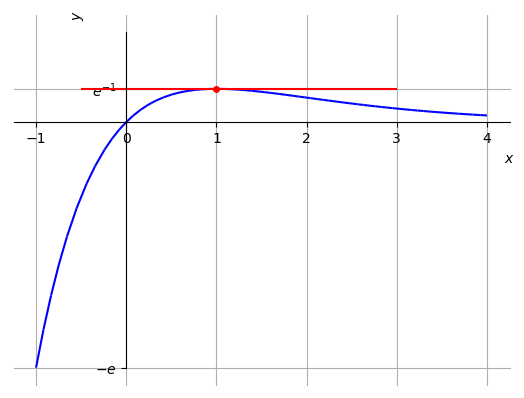
\includegraphics[width=0.7\textwidth]{fig_deriv/fig_deriv_exeresol_rt_xe-x}
    \caption{Esboço da reta tangente ao gráfico de $f(x)=xe^{-x}$ no ponto $x=1$.}
    \label{fig:deriv_exeresol_rt_xe-x}
  \end{figure}

  
  Com o \geogebra~ podemos computar a expressão desta reta tangente com os seguintes comandos:
\begin{verbatim}
f(x) = x*e^(-x)
x0 = 1
h(x) = derivada(f,x)
 y = h(1)*(x-1)+f(1)
\end{verbatim}
\vspace{-0.5cm}
\end{resol}

\subsection{Exercícios}

\begin{exer}
  Calcule a derivada em relação a $x$ das seguintes funções:
  \begin{enumerate}[a)]
  \item $f(x) = 2 - 5x^3$ 
  \item $g(x) = (2x-1)(2-4x^2)$
  \item $h(x) = \frac{2-4x^2}{2x-1}$
  \end{enumerate}
\end{exer}
\begin{resp}
  a) $f'(x) = -15x^2$; b)~$g'(x)=- 24 x^{2} + 8 x + 4$; c)~$\displaystyle h'(x) = \frac{4 \left(2 x^{2} - 2 x \left(2 x - 1\right) - 1\right)}{\left(2 x - 1\right)^{2}}$
\end{resp}

\begin{exer}
  Calcule a derivada em relação a $x$ das seguintes funções:
  \begin{enumerate}[a)]
  \item $f(x) = xe^x$
  \item $g(x) = xe^{2x}$
  \item $g(x) = xe^{-2x}$
  \end{enumerate}
\end{exer}
\begin{resp}
  a)~$f'(x) = (1+x)e^x$; b)~$g'(x) = (1+2x)e^{2x}$; c)~$h'(x) = (1-2x)e^{-2x}$
\end{resp}

\begin{exer}
  Calcule a derivada em relação a $x$ das seguintes funções:
  \begin{enumerate}[a)]
  \item $f(x) = \ln x^2$
  \item $g(x) = x\ln x^2$
  \item $g(x) = x\ln x^2e^x$
  \end{enumerate}
\end{exer}
\begin{resp}
  a)~$f'(x) = 2/x$; b)~$g'(x) = \ln x^2 + 2$; c)~$h'(x) = 2+2x+\ln x^2$
\end{resp}

\begin{exer}
  Encontre a equação da reta tangente ao gráfico de $f(x) = \ln x$ no ponto $x=1$.
\end{exer}
\begin{resp}
  $y = x-1$
\end{resp}

\section{Derivadas de funções trigonométricas}\label{cap:deriv_func_trig}

Começamos pela derivada da função seno. Pela definição da derivada, temos
\begin{align*}
  \sen' x &= \lim_{h\to 0} \frac{\sen(x+h) - \sen x}{h} \\
            &= \lim_{h\to 0} \frac{\sen(x)\cos(h)+\cos(x)\sen(h) - \sen x}{h} \\
            &= \lim_{h\to 0} \sen(x)\frac{\cos(h) - 1}{h} + \cos(x)\frac{\sen h}{h}\\
            &= \sen(x) \lim_{h\to 0} \frac{\cos(h)-1}{h} + \cos(x)\lim_{h\to 0} \frac{\sen h}{h}
\end{align*}
Usando do Teorema do confronto para limites de funções (recorrendo ao capítulo \ref{cap:limites}), podemos mostrar que
\begin{equation}
  \lim_{h\to 0} \frac{\sen h}{h} = 1\quad\text{e}\quad\lim_{h\to 0} \frac{\cos(h) - 1}{h} = 0
\end{equation}
Logo, temos
\begin{equation}
  \boldsymbol{\sen' x = \cos x}
\end{equation}

De forma similar, temos
\begin{align*}
  \cos' x &= \lim_{h\to 0} \frac{\cos(x+h) - \cos x}{h} \\
            &= \lim_{h\to 0} \frac{\cos(x)\cos(h)-\sen(x)\sen(h) - \cos x}{h} \\
            &= \lim_{h\to 0} \cos(x)\frac{\cos(h) - 1}{h} - \sen(x)\frac{\sen h}{h}\\
            &= \cos(x) \lim_{h\to 0} \cancelto{0}{\frac{\cos(h)-1}{h}} - \sen(x)\lim_{h\to 0} \cancelto{0}{\frac{\sen h}{h}}
\end{align*}
Ou seja,
\begin{equation}
  \boldsymbol{\cos' x = -\sen x}
\end{equation}

\begin{ex}
  A derivada de $f(x) = \sen^2 x + \cos^2 x$ é
  \begin{align*}
    f'(x) &= (\sen^2x + \cos^2 x)' \\
          &= (\sen^2 x)' + (\cos^2 x)' \\
          &= (\sen x\cdot \sen x)' + (\cos x\cdot \cos x)' \\
          &= \cos x\cdot \sen x + \sen x\cdot\cos x -\sen x\cdot \cos x - \cos x\cdot\sen x\\
          &= 0,
  \end{align*}
  conforme esperado.
\end{ex}

Conhecidas as derivadas da função seno e cosseno, podemos obter as derivadas das demais funções trigonométricas pela regra do quociente. Temos:
\begin{itemize}
\item $\boldsymbol{\tg' x = \sec^2 x}$

  Dem.:
  \begin{align*}
    \tg ' x &= \left(\frac{\sen x}{\cos x}\right)'\\
            &= \frac{\sen' x\cos x - \sen x\cos' x}{\cos^2 x} \\
            &= \frac{\cos x\cos x + \sen x\sen x}{\cos^2 x} \\
            &= \frac{1}{\cos^2 x} = \left(\frac{1}{\cos x}\right)^2 \\
            &= \sec^2 x
  \end{align*}

\item $\boldsymbol{\cotg' x = -\cossec^2 x}$

  Dem.:
  \begin{align*}
    \cotg ' x &= \left(\frac{\cos x}{\sen x}\right)'\\
            &= \frac{\cos' x\sen x - \cos x\sen' x}{\sen^2 x} \\
            &= \frac{-\sen x\sen x - \cos x\cos x}{\sen^2 x} \\
            &= \frac{-1}{\sen^2 x} = -\left(\frac{1}{\sen x}\right)^2 \\
            &= \cossec^2 x.
  \end{align*}

\item $\boldsymbol{\sec' x = \sec x\tg x}$

  Dem.:
  \begin{align*}
    \sec ' x &= \left(\frac{1}{\cos x}\right)'\\
            &= \frac{-\cos' x}{\cos^2 x} \\
            &= \frac{\sen x}{\cos^2 x} \\
            &= \frac{\sen x}{\cos x}\cdot \frac{1}{\cos x} \\
            &= \tg x\sec x
  \end{align*}

\item $\boldsymbol{\cossec' x = -\cossec x\cotg x}$

  Dem.:
  \begin{align*}
    \cossec ' x &= \left(\frac{1}{\sen x}\right)'\\
            &= \frac{-\sen' x}{\sen^2 x} \\
            &= \frac{-\cos x}{\sen^2 x} \\
            &= -\frac{\cos x}{\sen x}\cdot \frac{1}{\sen x} \\
            &= -\cotg x\cossec x
  \end{align*}
\end{itemize}

\begin{obs}
  Os cálculos acima, mostram que as funções trigonométricas são deriváveis em todos os pontos de seus domínios.
\end{obs}

\begin{ex}
  A derivada em relação a $x$ de
  \begin{equation*}
    f(x) = \frac{x + \tg x}{\sec x}
  \end{equation*}
  pode ser calculada como segue
  \begin{align*}
    f'(x) &= \left(\frac{x+\tg x}{\sec x}\right)' \\
          &= \frac{(x+\tg x)'\sec x - (x+\tg x)\sec' x}{\sec^2 x} \\
          &= \frac{(1+\sec^2 x)\sec x - (x+\tg x)\sec x\tg x}{\sec^2 x} \\
          &= \frac{1+\sec^2 x - (x+\tg x)\tg x}{\sec x}
  \end{align*}

  
  Com o \geogebra~ podemos computar esta derivada com o seguinte comando:
\begin{verbatim}
derivada((x+tan(x))/sec(x),x)
\end{verbatim}

\end{ex}

\subsection{Tabela de derivadas}

\begin{align*}
  & (ku)' = ku' && (u\pm v)' = u' \pm v'\\
  & (uv)' = u'v + uv' && \left(\frac{u}{v}\right)' = \frac{u'v - uv'}{v^2} \\
  & (k)' = 0 && (x^n)' = nx^{n-1}\\
  & (a^x)' = a^x\ln a && (e^x)' = e^x \\
  & \sen' x = \cos x && \cos' x = - \sen x\\
  & \tg' x = \sec^2 x && \cotg' x = -\cossec^2 x \\
  & \sec' x = \sec x \tg x && \cossec' x = -\cossec x\cotg x
\end{align*}

\subsection{Exercícios resolvidos}

\begin{exeresol}
  Encontre a equação da reta tangente ao gráfico da função $y = \sen x$ no ponto $x=0$. Então, faça os esboços desta função e da reta tangente, em uma mesma figura.
\end{exeresol}
\begin{resol}
  A equação da reta tangente ao gráfico de uma função $y = f(x)$ no ponto $x=x+0$ é
  \begin{equation*}
    y = f'(x_0)(x-x_0)+f(x_0)
  \end{equation*}
  No caso deste exercício, temos $f(x)=\sen x$ e $x_0=0$. Assim sendo, calculamos a derivada em relação a $x$ de $f(x)$, i.e.
  \begin{equation*}
    f'(x) = \sen' x = \cos x
  \end{equation*}
  Segue que a equação da reta tangente é
  \begin{align*}
    y = f'(0)(x-0)+f(0) &\Rightarrow y = \cos(0)(x-0)+\sen(0) \\
                        &\Rightarrow y = x
  \end{align*}
  Na Figura \ref{fig:deriv_exeresol_rt_sen0}, temos os esboços dos gráficos da função seno e da reta tangente encontrada.

  \begin{figure}[H]
    \centering
    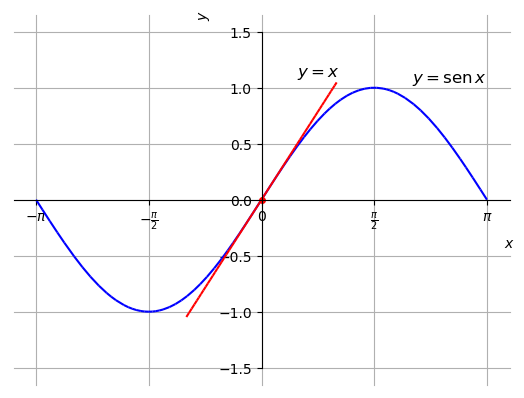
\includegraphics[width=0.65\textwidth]{fig_deriv/fig_deriv_exeresol_rt_sen0}
    \caption{Esboços dos gráfico da função seno e de sua reta tangente no ponto $x=0$.}
    \label{fig:deriv_exeresol_rt_sen0}
  \end{figure}
\end{resol}

\begin{exeresol}
  Resolva a equação
  \begin{equation*}
    \sec'(x) = 0
  \end{equation*}
  para $x\in \left(\frac{\pi}{2}, \frac{3\pi}{2}\right)$.\\
\end{exeresol}

\begin{resol}
  Temos
  \begin{align*}
    \sec'(x) = 0 &\Rightarrow \sec(x)\tg(x) = 0 \\
                 &\Rightarrow \frac{1}{\cos(x)}\frac{\sen(x)}{\cos(x)} = 0 \\
                 &\Rightarrow \frac{\sen(x)}{\cos^2(x)} = 0 \\
                 &\Rightarrow \sen(x) = 0
  \end{align*}
  Para $x\in \left(\frac{\pi}{2}, \frac{3\pi}{2}\right)$, a função seno se anula somente em $x=\pi$, a qual é a solução da equação.
\end{resol}


\subsection{Exercícios}

\begin{exer}
  Calcule a derivada em relação a $x$ de
  \begin{enumerate}[a)]
  \item $\displaystyle f(x)=\sen(x)-\cos^2(x)$
  \item $\displaystyle g(x)=\sen^2(x)\cos(x)$
  \item $\displaystyle h(x)=\frac{2\tg(x)}{\sec(x)}$
  \end{enumerate}
\end{exer}
\begin{resp}
  a)~$f'(x)=\sen(2x)+\cos(x)$; b)~$g'(x)=\sen(x)\cdot(2-3\sin^2(x)))$; c)~$h'(x)=2\cos(x)$
\end{resp}

\begin{exer}
  Encontre a equação da reta tangente ao gráfico da função $y = \cos x$ no ponto $x=0$. Então, faça os esboços desta função e da reta tangente, em uma mesma figura.  
\end{exer}
\begin{resp}
  $y = 1$. Dica: use um pacote de matemática simbólica para verificar os esboços dos gráficos.
\end{resp}

\begin{exer}
  Calcule a derivada em relação a $x$ de
  \begin{enumerate}[a)]
  \item $\displaystyle f(x)=\tg(x)-\cotg(x)$
  \item $\displaystyle g(x)=\sec(x)-\cossec(x)$
  \item $\displaystyle g(x)=\sec(x)-\cossec(x)$
  \end{enumerate}
\end{exer}
\begin{resp}
  a)~$f'(x)=\sec^2(x)+\cossec^2(x)$; b)~$g'(x)=\sec(x)\tg(x)+\cossec(x)\cotg(x)$; c)~$h'(x)=\frac{1}{2}\sec^2(x)$
\end{resp}


\section{Regra da cadeia}\label{Chap:RegraCadeia}
Regra da cadeia é nome dado a técnica de derivação de uma função composta. Sejam $f$ e $g$, com $g$ derivável em $x$ e $f$ derivável em $g(x)$, então $(f\circ g)$ é derivável em $x$, sendo
\begin{equation}
  \boldsymbol{(f\circ g)'(x) = [f(g(x))]' = f'(g(x))\cdot g'(x)},
\end{equation}
chamada de regra da cadeia.

\begin{ex}
  A derivada em relação a $x$ de $h(x) = (x+1)^2$ pode ser calculada das seguintes formas:
  \begin{enumerate}
  \item[a)] pela regra da cadeia.
  
\begin{solution}
    A função $h$ é a composição da função $f(x)=x^2$ com a função $g(x)=x+1$, i.e. $h(x) = f(g(x))$. Temos $f'(x)=2x$ e $g'(x)=1$. Então, segue pela regra da cadeia
    \begin{align*}
      h'(x) &= [f(g(x))]' \\
            &= f'(g(x))\cdot g'(x) \\
            &= 2(x+1)\cdot 1 \\
            &= 2x+2
    \end{align*}
\end{solution}
  \item[b)] por cálculo direto.
  
\begin{solution}
    Observando que $h(x)=(x+1)^2=x^2+2x+1$, temos
    \begin{align*}
      h'(x) &= (x^2+2x+1)' \\
            &= (x^2)' + (2x)' + (1)' \\
            &= 2x + 2
    \end{align*}
      \end{solution}
  \end{enumerate}
\end{ex}

Usualmente, a regra da cadeia também é apresentada da seguinte forma
\begin{equation*}\label{eq:deriv_regra_da_cadeia}
  \boldsymbol{\frac{\dd}{\dd x}f(u) = f'(u)\frac{\dd u}{\dd x}}
\end{equation*}
onde $u$ é uma função derivável em $x$ e $f$ é derivável em $u(x)$.

\begin{ex}~
  Vamos calcular a derivada em relação a $x$ de $g(x) = \sqrt{x^2+1}$. Temos que $g(x) = f(u(x))$, com $f(x) = \sqrt{x}$ e $u(x) = x^2+1$. Observando que
  \begin{equation}
    f'(x) = \frac{1}{2\sqrt{x}}\quad\text{e}\quad u'(x)=2x
  \end{equation}
  \begin{solution}
  segue pela regra da cadeia que
  \begin{align*}
    g'(x) &= \frac{\dd}{\dd x}f(u) \\
          &= f'(u)\frac{\dd u}{\dd x} \\
          &= \frac{1}{2\sqrt{u}}\cdot 2x \\
          &= \frac{x}{\sqrt{x^2+1}}
  \end{align*}
  \end{solution}
\end{ex}

A regra da cadeia pode ser estendida para calcular a derivada de uma composição encadeada de três ou mais funções. Por exemplo,
\begin{equation}
  [f(g(h(x)))]' = f'(g(h(x)))\cdot[g(h(x))]' = f'(g(h(x)))\cdot g'(h(x))\cdot h'(x)
\end{equation}
Neste caso, a regra é válida para todo ponto tal que $h$ é derivável em $x$ com $g$ derivável em $h(x)$ e $f$ derivável em $f(g(h(x)))$.

\begin{ex}
  Vamos calcular a derivada em relação a $x$ de $f(x) = \sen(\cos(x^2))$. Pela regra da cadeia, temos
  \begin{align*}
    [\sen(\cos(x^2))] &= \cos(\cos(x^2))\cdot[\cos(x^2)]' \\
                    &= \cos(\cos(x^2))\cdot [-\sen(x^2)\cdot (x^2)'] \\
                    &= -\cos(\cos(x^2))\cdot\sen(x^2)\cdot 2x
  \end{align*}
\end{ex}

\subsection{Tabela de derivadas}

\begin{align}
  & (ku)' = ku' && (u\pm v)' = u' \pm v'\\
  & (uv)' = u'v + uv' && \left(\frac{u}{v}\right)' = \frac{u'v - uv'}{v^2} \\
  & (k)' = 0 && \frac{\dd}{\dd x}u^n = nu^{n-1}\frac{\dd u}{\dd x}\\
  & \frac{\dd}{\dd x}a^u = a^u\ln a\frac{\dd u}{\dd x} && \frac{\dd}{\dd x}(e^u) = e^u\frac{\dd u}{\dd x} \\
  & \frac{\dd}{\dd x}\sen u = \cos(u)\frac{\dd u}{\dd x} && \frac{\dd}{\dd x}\cos u = - \sen(u)\frac{\dd u}{\dd x}\\
  & \frac{\dd}{\dd x}\tg u = \sec^2(u)\frac{\dd u}{\dd x} && \frac{\dd}{\dd x}\cotg u = -\cossec^2(u)\frac{\dd u}{\dd x} \\
  & \frac{\dd}{\dd x}\sec u = \sec(u)\tg(u)\frac{\dd u}{\dd x} && \frac{\dd}{\dd x}\cossec u = -\cossec(u)\cotg(u)\frac{\dd u}{\dd x}
\end{align}

\subsection{Exercícios resolvidos}

\begin{exeresol}
  Calcule a derivada em relação a $x$ de
  \begin{equation*}
    f(x) = e^{\sqrt{x+1}}
  \end{equation*}
\end{exeresol}
\begin{resol}
  Da regra da cadeia aplicada à função exponencial, temos
  \begin{equation*}
    \frac{\dd}{\dd x}e^u = e^u\frac{\dd u}{\dd x}
  \end{equation*}
  Então, com $u = \sqrt{x+1}$, segue
  \begin{align*}
    f'(x) &= \frac{\dd}{\dd x}e^{\sqrt{x+1}} \\
          &= e^{\sqrt{x+1}}\frac{\dd}{\dd x}\left(\sqrt{x+1}\right)
  \end{align*}
  Agora, aplicamos a regra da cadeia para a função raiz quadrada, i.e.
  \begin{equation*}
    \frac{\dd}{\dd x}\sqrt{u} = \frac{1}{2\sqrt{u}}\frac{\dd u}{\dd x}
  \end{equation*}
  com $u = x+1$. Segue, então
  \begin{align*}
    \frac{\dd}{\dd x}\sqrt{x+1} &= \frac{1}{2}(x+1)^{\frac{1}{2}-1}\frac{\dd}{\dd x}(x+1) \\
                                &= \frac{1}{2\sqrt{x+1}}
  \end{align*}
  Portanto, concluímos que
  \begin{equation*}
    f'(x) = \frac{1}{2\sqrt{x+1}}e^{\sqrt{x+1}}
  \end{equation*}
\end{resol}

\begin{exeresol}
  Mostre que a função logística
  \begin{equation*}
    f(x) = \frac{1}{1+e^{-x}}
  \end{equation*}
  satisfaz a equação diferencial
  \begin{equation*}
    \frac{\dd}{\dd x}f(x) = f(x)(1-f(x))
  \end{equation*}
\end{exeresol}
\begin{resol}
  Vamos calcular a derivada em relação a $x$ da função logística, i.e.
  \begin{align*}
    \frac{\dd}{\dd x}f(x) &= \frac{\dd}{\dd x}\left(\frac{1}{1+e^{-x}}\right) \\
          &= \frac{\dd}{\dd x}\left[\left(1+e^{-x}\right)^{-1}\right] \\
          &= -1\cdot\left(1+e^{-x}\right)^{-2}\cdot\underbrace{\left(1+e^{-x}\right)'}_{=-e^{-x}} \\
          &= \frac{e^{-x}}{\left(1+e^{-x}\right)^{2}}
  \end{align*}
  Por outro lado, temos
  \begin{align*}
    f(x)(1-f(x)) &= \frac{1}{1+e^{-x}}\cdot\left(1 - \frac{1}{1+e^{-x}}\right) \\
                 &= \frac{1}{1+e^{-x}}\cdot\left(\frac{1+e^{-x}-1}{1+e^{-x}}\right) \\
                 &= \frac{e^{-x}}{\left(1+e^{-x}\right)^{2}}
  \end{align*}
  Ou seja, de fato temos
  \begin{equation*}
    \frac{\dd}{\dd x}f(x) = f(x)(1-f(x))
  \end{equation*}  
\end{resol}

\begin{exeresol}
  Assuma que o custo de produção de uma unidade empresarial seja modelada pela função
  \begin{equation*}
    c(x) = \sqrt{x-1} + e^{x-7}
  \end{equation*}
  onde $c$ é o custo em função da produção $x$. Determine o custo marginal quando $x=3$.
\end{exeresol}
\begin{resol}
  O custo marginal é a função derivada do custo em relação à produção. Calculando, temos
  \begin{align*}
    c'(x) &= \left(\sqrt{x-1} + e^{x-7}\right)\\
          &= \underbrace{\left(\sqrt{x-1}\right)'}_{(u^n)' = nu^{n-1}u'} + \underbrace{\left(e^{x-7}\right)'}_{(e^u)' = e^uu'}\\
          &= \frac{1}{2\sqrt{x-1}} + e^{x-7}
  \end{align*}
  Logo, o custo marginal quando $x=3$ é
  \begin{equation*}
    c'(3) = \frac{1}{2\sqrt{3-1}} + e^{3-7} = \sqrt{2} + e^{-4}
  \end{equation*}
\end{resol}

\subsection{Exercícios}

\begin{exer}
  Calcule a derivada em relação a $x$ das seguintes funções
  \begin{enumerate}[a)]
  \item $\displaystyle f(x) = (2x-3)^{9}$
  \item $\displaystyle g(x) = \frac{1}{(2x-3)^{51}}$
  \end{enumerate}
\end{exer}
\begin{resp}
  a)~$\displaystyle f'(x) = 18(2x-3)^8$; b)~$\displaystyle g'(x) = -\frac{102}{(2x-3)^{52}}$;
\end{resp}

\begin{exer}
  Calcule a derivada em relação a $x$ das seguintes funções
  \begin{enumerate}[a)]
  \item $\displaystyle f(x) = 2^{3x-1}$
  \item $\displaystyle g(x) = e^{-x^2}$
  \end{enumerate}
\end{exer}
\begin{resp}
  a)~$\displaystyle f'(x) = 3\cdot 2^{3x-1}\ln 2$; b)~$\displaystyle g'(x) = -2xe^{-x^2}$.
\end{resp}

\begin{exer}
  Calcule a derivada em relação a $x$ das seguintes funções
  \begin{multicols}{2}
   \begin{enumerate}[a)]
  \item $\displaystyle f(x) = \sen(\pi x)$
  \item $\displaystyle g(x) = \cos(\sqrt{x})$
  \item $\displaystyle h(x) = \tg(2x)$
  \item $\displaystyle u(x) = \cotg(3 - x)$
  \item $\displaystyle v(x) = \sec\left(\frac{1}{x^2}\right)$
  \item $\displaystyle z(x) = \cossec\left(5x + x^2\right)$
  \end{enumerate}
  \end{multicols}
 
\end{exer}
\begin{resp}
  a)~$\displaystyle f'(x) = \pi\cos(\pi x)$; b)~$\displaystyle g'(x) = -\frac{1}{2\sqrt{x}}\sen(\sqrt{x})$; c)~$\displaystyle h'(x) = 2\sec^2(2x)$; d)~$\displaystyle u'(x) = \cossec^2(3-x)$; e)~$\displaystyle v'(x) = -\frac{2}{x^2}\sec\left(\frac{1}{x^2}\right)\tg\left(\frac{1}{x^2}\right)$; f)~$\displaystyle z'(x) = -(5+2x)\cossec\left(5x + x^2\right)\cotg\left(5x + x^2\right)$
\end{resp}

\section{Diferenciabilidade da função inversa}\label{Chap:DerivFuncInversa}

Seja $f$ uma função diferenciável e injetora em um intervalo aberto $I$. Então, pode-se mostrar que sua inversa $f^{-1}$ é diferenciável em qualquer ponto da imagem da $f$ no qual $f'(f^{-1}(x))\neq 0$ e sua derivada é
\begin{equation}
  \boldsymbol{\frac{d}{dx}[f^{-1}(x)] = \frac{1}{f'(f^{-1}(x))}}\label{eq:DerivFuncInversa}
\end{equation}

\begin{ex}
  Seja $f(x) = (2x-1)^2$ para $x>1/2$. Para calcular sua inversa, fazemos
  \begin{align*}
    y = (2x-1)^2 &\Rightarrow \sqrt{y} = 2x-1\\
               &\Rightarrow x = \frac{\sqrt{y}+1}{2}
  \end{align*}
  Ou seja,
  \begin{equation*}
    f^{-1}(x) = \frac{1}{2}(\sqrt{x}+1)
  \end{equation*}
  Calculando a derivada de $f^{-1}$ diretamente, temos
  \begin{align*}
    \frac{\dd}{\dd x}f^{-1}(x) &= \frac{1}{2}\left(\sqrt{x}+1\right)' \\
                               &= \frac{1}{2}\cdot\frac{1}{2\sqrt{x}} \\
                               &= \frac{1}{4\sqrt{x}}
  \end{align*}
  Agora, usando \ref{eq:DerivFuncInversa} e observando que $f'(x) = 8x-4$, obtemos
  \begin{align*}
    \frac{\dd}{\dd x}f^{-1}(x) &= \frac{1}{f'(f^{-1}(x))}\\
                               &= \frac{1}{8\cdot \frac{1}{2}\left(\sqrt{x}+1\right)-4} \\
                               &= \frac{1}{4\sqrt{x}}
  \end{align*}
  como esperado.
\end{ex}

\begin{obs}\normalfont{(Derivada da função logarítmica)}
  \begin{itemize}
  \item Tomando $f(x) = e^x$ temos $f^{-1}(x) = \ln x$ e, daí por \ref{eq:DerivFuncInversa}
    \begin{equation}
      \frac{\dd }{\dd x}\ln x = \frac{1}{e^{\ln x}} = \frac{1}{x}
    \end{equation}
  \item Tomando $f(x) = a^x$, $a> 0$ e $a\neq 1$, temos $f^{-1}(x) = \log_a x$ e, por \ref{eq:DerivFuncInversa},
    \begin{equation}
      \frac{\dd}{\dd x}\log_a x = \frac{1}{a^{\log_a x}\ln a} = \frac{1}{x\ln a}.
    \end{equation}
  \end{itemize}
\end{obs}

\begin{ex}
  Vamos calcular a derivada em relação a $x$ da função
  \begin{equation}
    f(x) = \ln \frac{1}{x}
  \end{equation}
  Aplicando a regra da cadeia na derivada da função logarítmica, temos
  \begin{equation}
    \frac{\dd}{\dd x}\ln u = \frac{1}{u}\frac{\dd u}{\dd x}
  \end{equation}
  Portanto, temos
  \begin{align*}
    f'(x) &= \left(\ln\frac{1}{x}\right)'\\
          &= \frac{1}{x^{-1}}\cdot (-x^{-2}) \\
          &= -\frac{1}{x}
  \end{align*}
\end{ex}

\begin{obs}\normalfont{(Derivada de função potência)}
  Em seções anteriores, já vimos que
  \begin{equation}
    \frac{\dd}{\dd x}x^n = nx^{n-1}
  \end{equation}
  para qualquer $n$ inteiro\footnote{Mais precisamente, para $n\neq 0$ e $n\neq 1$.}. Agora, se $r\neq 0$ e $r\neq 1$ é um número real, temos
  \begin{equation}
    y = x^r \Rightarrow \ln y = \ln x^r = r\ln x.
  \end{equation}
  Daí, derivando ambos os lados desta última equação e observando que $y = y(x)$, obtemos
  \begin{align*}
    \frac{\dd}{\dd x} \ln y = \frac{\dd}{\dd x} r\ln x &\Rightarrow \frac{1}{y}\frac{\dd y}{\dd x} = \frac{r}{x}\\
                                                       &\Rightarrow \frac{\dd y}{\dd x} = \frac{r}{x}y\\
                                                       &\Rightarrow \frac{\dd y}{\dd x} = rx^{r-1}
  \end{align*}
  Ou seja, a regra da potência
  \begin{equation}
    \frac{\dd}{\dd x}x^r = rx^{r-1}
  \end{equation}
  vale para todo $r$ real, com $r\neq 0$ e $r\neq 1$
\end{obs}

\begin{ex}
  Vejamos os seguintes casos:
  \begin{enumerate}[a)]
  \item
    \begin{align*}
      \frac{\dd}{\dd x}\sqrt{x} &= \left(x^{\frac{1}{2}}\right)' \\
                                &= \frac{1}{2}x^{\frac{1}{2}-1} \\
                                &= \frac{1}{2\sqrt{x}}
    \end{align*}
  \item
    \begin{align}
      \left(x^{\sqrt{2}}\right)' = \sqrt{2}x^{\sqrt{2}-1}
    \end{align}
  \end{enumerate}
\end{ex}

\begin{ex}
  A regra da cadeia aplicada a derivada da função potência é
  \begin{equation*}
    \frac{\dd}{\dd x}u^r = ru^{r-1}\frac{\dd u}{\dd x}.
  \end{equation*}
  
  Por exemplo, temos
  \begin{align*}
    \frac{\dd}{\dd x}\sqrt[3]{(x^2-1)} &= \frac{\dd}{\dd x}(x^2-1)^{\frac{1}{3}} \\
                                       &= \frac{2}{3}x\cdot (x^2-1)^{\frac{1}{3}-1} \\
                                       &= \frac{2}{3}x\cdot (x^2-1)^{-\frac{2}{3}} \\
                                       &= \frac{2x}{3\sqrt[3]{(x^2-1)^2}}
  \end{align*}
\end{ex}
\subsection{Exercícios Resolvidos}
\begin{exeresol}
  Seja \(f(x)=x^3-7\). Determine o valor de \((f^{-1})'\) em \(x=20\)\\
  \begin{resol}
    Aplicamos a Fórmula \ref{eq:DerivFuncInversa} para obter o valor de \((f^{-1})'\) em \(x=20\). De fato, observamos que \(20=f(3)\), o que resulta em \(f^{-1}(20)=3\) e

\[ f'(x)=3x^2 \quad \Rightarrow \quad f'(3)=3(3)^2=27. \]
Portanto,

\[ \left(f^{-1}\right)'(20)= \dfrac{1}{f'\left(f^{-1}(20) \right)} = \dfrac{1}{f'(3)} =\dfrac{1}{27}. \]
  \end{resol}
\end{exeresol}
\begin{exeresol}
  Seja \(f(x)=x^2+2x+3\) com domínio \({\rm Dom}(f)=[-1,+\infty)\). Determine o valor de \((f^{-1})'\) em \(x=6\).\\
  \begin{resol}
    Aplicamos a Fórmula \ref{eq:DerivFuncInversa}  para obter o valor de \((f^{-1})'\) em \(x=6\). De fato, devemos identificar a \(f^{-1}(6)\)

\[ 6=f(x)=x^2+2x+3 \quad \Rightarrow \quad x^2+2x-3=0 \quad \mbox{obtemos} \quad x=-3,\quad x=1; \]
porém como somente deve existir uma única solução, descartamos \(x=-3\), pois \(-3\not\in{\rm Dom}(f)=[-1,+\infty)\). Assim \(1=f^{-1}(6)\), alem disso

\[ f'(x)=2x+2 \quad \Rightarrow \quad f'(1)=2(1)+2=4 \]
Portanto,

\[ \left(f^{-1}\right)'(6)= \dfrac{1}{f'\left(f^{-1}(6) \right)} = \dfrac{1}{f'(1)} =\dfrac{1}{4}. \]
  \end{resol}
\end{exeresol}
\subsection{Derivadas de funções trigonométricas inversas}

Seja $f(x) = \sen x$ restrita a $-\pi/2 \leq x \leq \pi/2$. Sua inversa é a função arco seno, denotada por
\begin{equation}
  y = \arc\sen x.
\end{equation}

\begin{figure}[H]
  \centering
  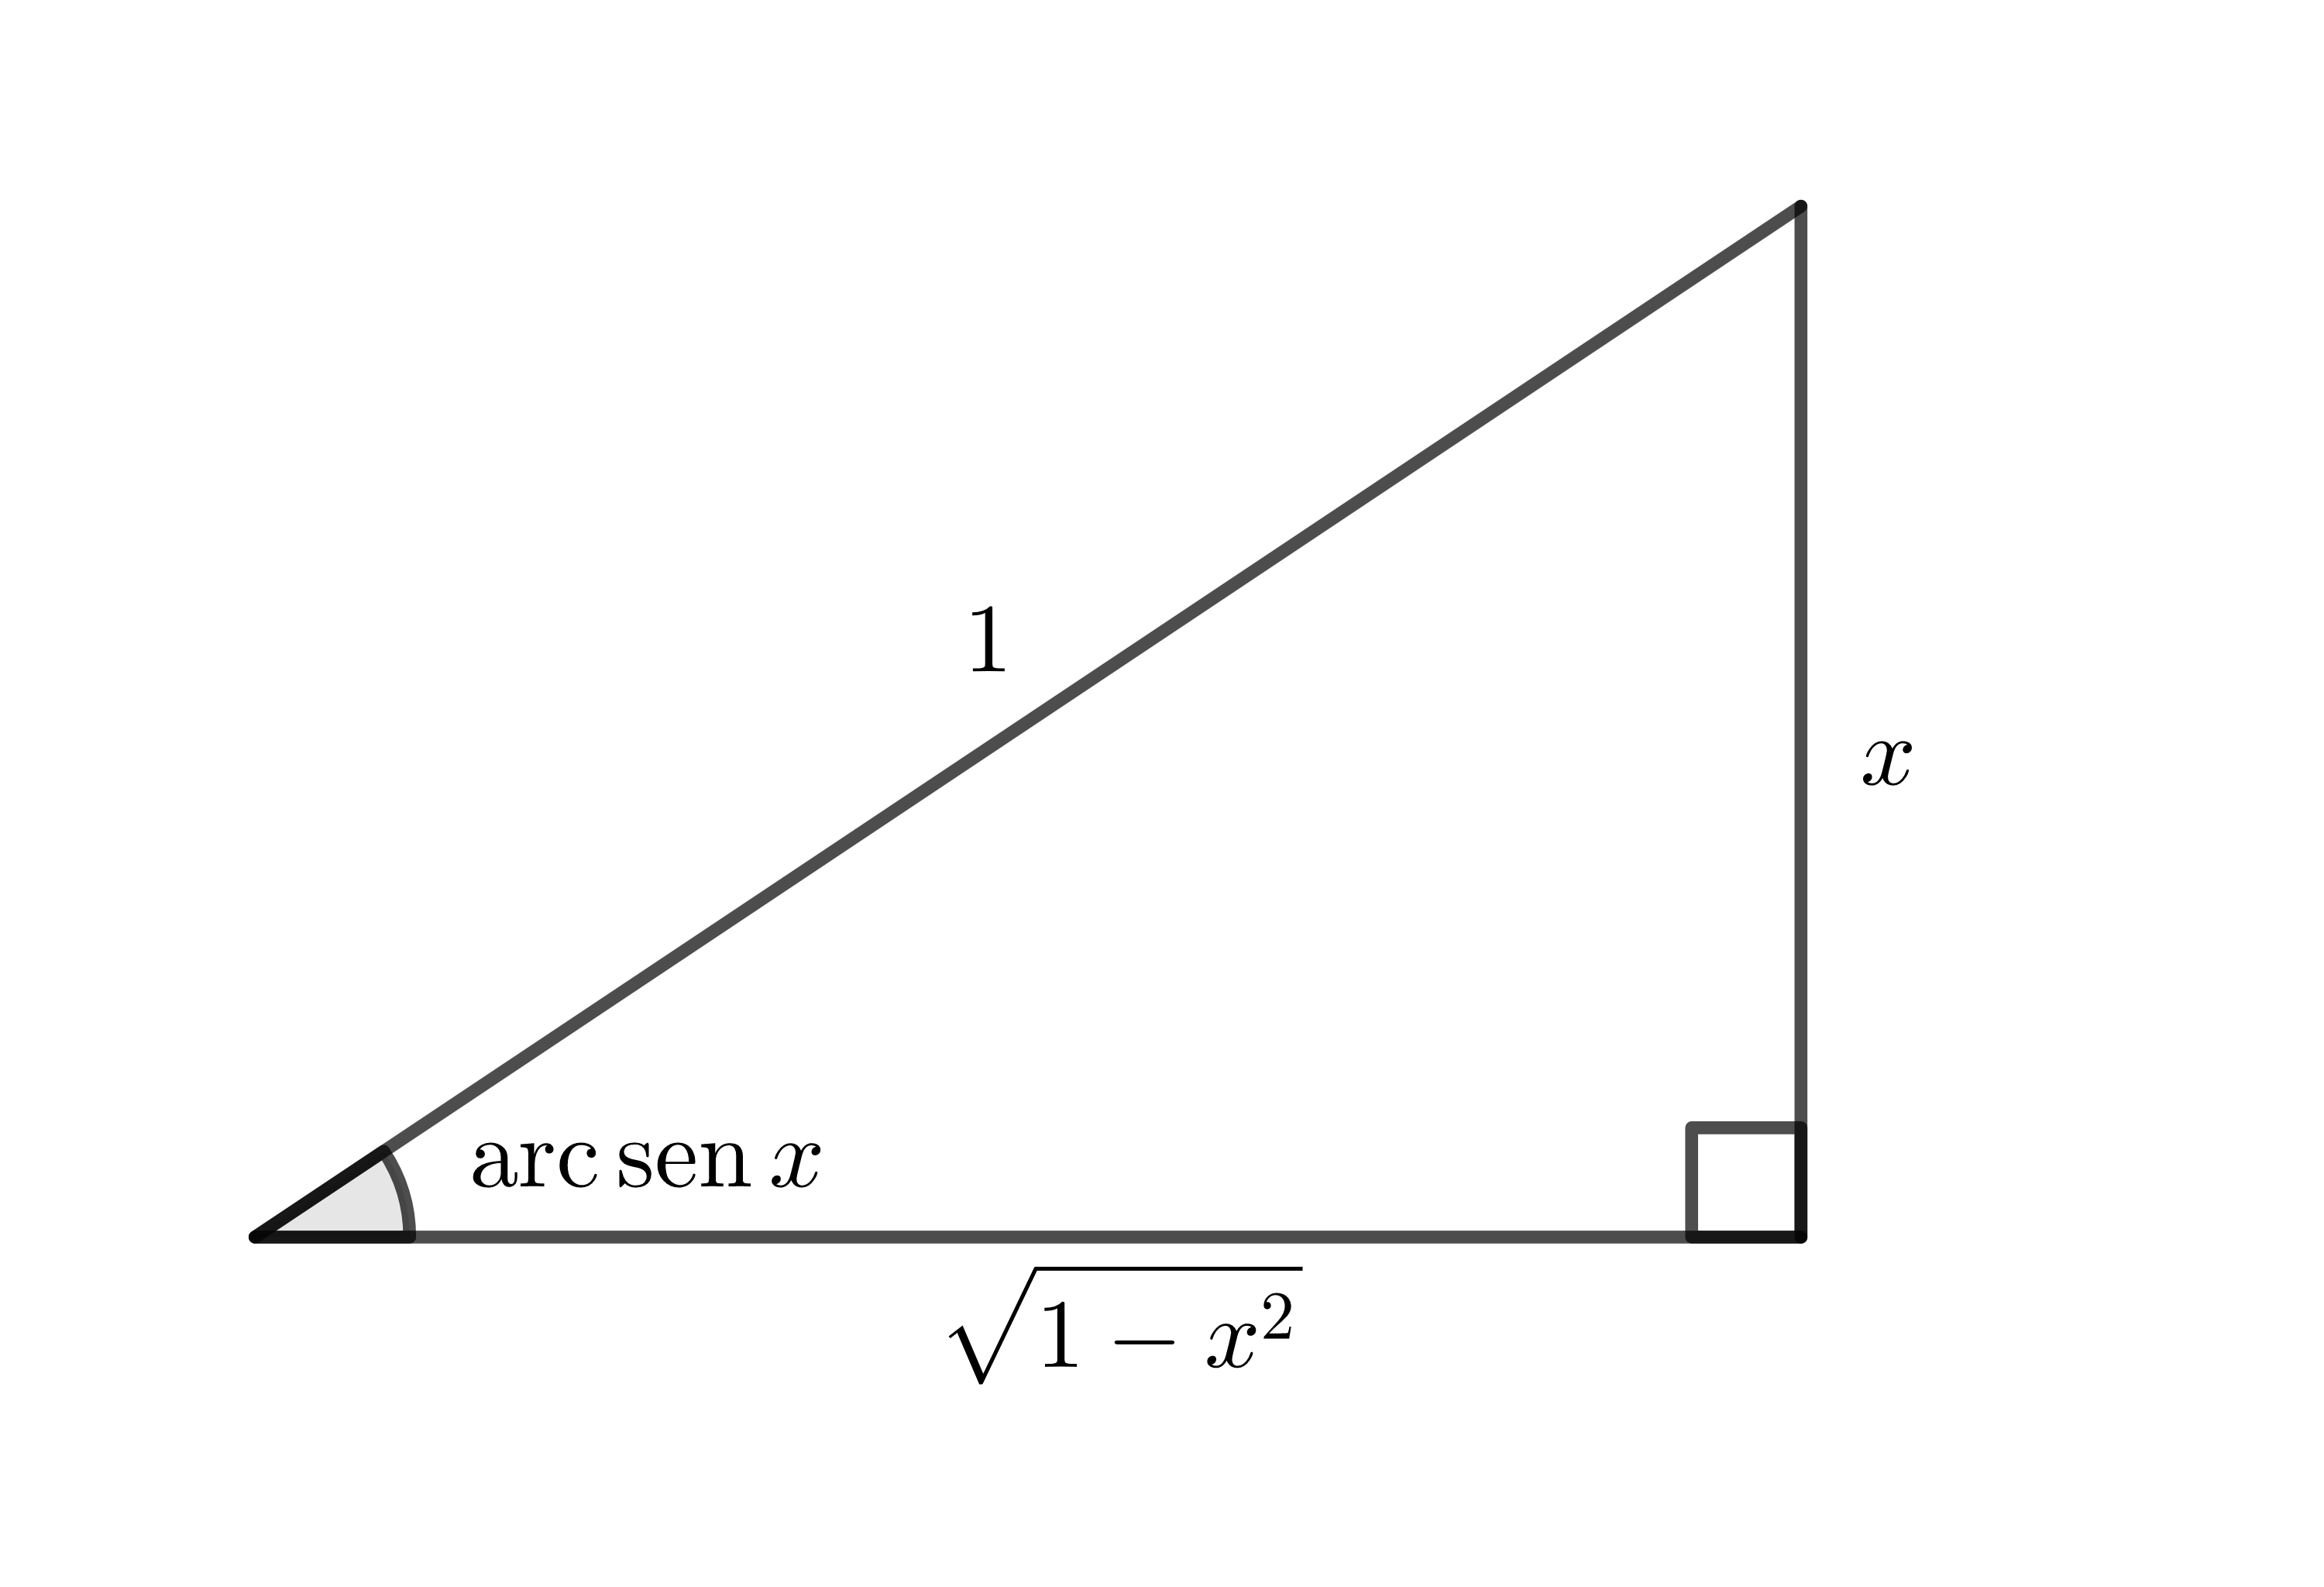
\includegraphics[width=0.5\textwidth]{fig_deriv/fig_diff_arc_sen}
  \caption{Arco seno de um ângulo no triângulo retângulo.}
  \label{fig:diff_arc_sen}
\end{figure}

Para calcular a derivada da função arco seno, vamos usar a Equação \ref{eq:DerivFuncInversa} com $f(x)=\sen x$ e $f^{-1}(x) = \arc\sen x$, donde
\begin{equation}
  (\arc\sen x)' = \frac{1}{\cos(\arc\sen x)}
\end{equation}
Como $\cos(\arc\sen x) = \sqrt{1-x^2}$ (veja Figura \ref{fig:diff_arc_sen}), concluímos
\begin{equation}
  (\arc\sen x)' = \frac{1}{\sqrt{1-x^2}}
\end{equation}


\begin{ex}
  A regra da cadeia aplicada à derivada da função arco seno é
  \begin{equation}
    \frac{\dd}{\dd x}\arc\sen u = \frac{1}{\sqrt{1-u^2}}\frac{\dd u}{\dd x}
  \end{equation}

  Por exemplo, temos
  \begin{equation}
    \frac{\dd}{\dd x}\arc\sen x^2 = \frac{2x}{\sqrt{1-x^4}}
  \end{equation}

  
  No \geogebra~ temos o seguinte comando \verb=derivada(asin(x**2),x)=
\end{ex}

Com argumentos análogos aos usados no cálculo da derivada da função arco seno, podemos obter as seguintes derivadas (\dica experimente!):
\begin{align*}
  & (\arc\cos x)' = -\frac{1}{\sqrt{1-x^2}} && \\
  &(\arc\tg x)' = \frac{1}{1+x^2} && (\arc\cotg x)' = -\frac{1}{1+x^2} \\
  & (\arc\sec x)' = \frac{1}{|x|\sqrt{x^2-1}} && (\arc\cosec x)' = -\frac{1}{|x|\sqrt{x^2-1}}
\end{align*}

\begin{ex}
  A regra da cadeia aplicada a função arco tangente é
  \begin{equation}
    \frac{\dd}{\dd x}\arc\tg u = \frac{1}{1+u^2}\frac{\dd u}{\dd x}.
  \end{equation}

  Por exemplo, temos
  \begin{align*}
    \frac{\dd}{\dd x}\arc\tg\sqrt{x} &= \frac{1}{1+(\sqrt{x})^2}\frac{\dd}{\dd x}\sqrt{x} \\
                                     &=  \frac{1}{2(1+x)\sqrt{x}}.
  \end{align*}

  
  No \geogebra~ podemos utilizar o comando:
\begin{verbatim}
derivada(atan(sqrt(x)))
\end{verbatim}
    
\end{ex}

\subsection{Tabela de derivadas}\label{deriv_tabela_de_derivadas}

\begin{small}
\begin{align}
  & (ku)' = ku' && (u\pm v)' = u' \pm v'\\
  & (uv)' = u'v + uv' && \left(\frac{u}{v}\right)' = \frac{u'v - uv'}{v^2} \\
  & (k)' = 0 && \frac{\dd}{\dd x}u^r = ru^{r-1}\frac{\dd u}{\dd x}\\
  & \frac{\dd}{\dd x}a^u = a^u\ln a\frac{\dd u}{\dd x} && \frac{\dd}{\dd x}e^u = e^u\frac{\dd u}{\dd x} \\
  & \frac{\dd}{\dd x}\log_a u = \frac{1}{u\ln a}\frac{\dd u}{\dd x} && \frac{\dd}{\dd x}\ln u = \frac{1}{u}\frac{\dd u}{\dd x} \\
  & \frac{\dd}{\dd x}\sen u = \cos(u)\frac{\dd u}{\dd x} && \frac{\dd}{\dd x}\cos u = - \sen(u)\frac{\dd u}{\dd x}\\
  & \frac{\dd}{\dd x}\tg u = \sec^2(u)\frac{\dd u}{\dd x} && \frac{\dd}{\dd x}\cotg u = -\cossec^2(u)\frac{\dd u}{\dd x} \\
  & \frac{\dd}{\dd x}\sec u = \sec(u)\tg(u)\frac{\dd u}{\dd x} && \frac{\dd}{\dd x}\cossec u = -\cossec(u)\cotg(u)\frac{\dd u}{\dd x} \\
  &\frac{\dd}{\dd x}\arc\sen u = \frac{1}{\sqrt{1-u^2}}\frac{\dd u}{\dd x} && \frac{\dd}{\dd x}\arc\cos u = -\frac{1}{\sqrt{1-u^2}}\frac{\dd u}{\dd x} \\
  &\frac{\dd}{\dd x}\arc\tg u = \frac{1}{1+u^2}\frac{\dd u}{\dd x} && \frac{\dd}{\dd x}\arc\cotg u = -\frac{1}{1+u^2}\frac{\dd u}{\dd x} \\
  &\frac{\dd}{\dd x}\arc\sec u = \frac{1}{|u|\sqrt{u^2-1}}\frac{\dd u}{\dd x} && \frac{\dd}{\dd x}\arc\cossec u = -\frac{1}{|u|\sqrt{u^2-1}}\frac{\dd u}{\dd x}
\end{align}
\end{small}

\subsection{Exercícios resolvidos}

\begin{exeresol}
  Calcule a equação da reta tangente ao gráfico da função $f(x) = \ln x$ no ponto $x=1$. Faça, então, um esboço dos gráficos da função e da reta tangente.
\end{exeresol}
\begin{resol}
  A equação da reta tangente ao gráfico da função $f(x) = \ln x$ no ponto $x_0=1$ é
  \begin{equation*}
    y = f'(x_0)(x-x_0)+f(x_0) \Rightarrow y = f'(1)(x-1)+f(1)
  \end{equation*}
  Observando que
  \begin{equation*}
    f'(x) = (\ln x)' = \frac{1}{x}
  \end{equation*}
  temos que a equação da reta tangente é
  \begin{equation*}
    y = \frac{1}{1}(x-1)+\ln 1 \Rightarrow y = x-1
  \end{equation*}
  Na Figura \ref{fig:deriv_exeresol_rt_ln}, temos um esboço dos gráficos da função e da reta tangente.

  \begin{figure}[H]
    \centering
    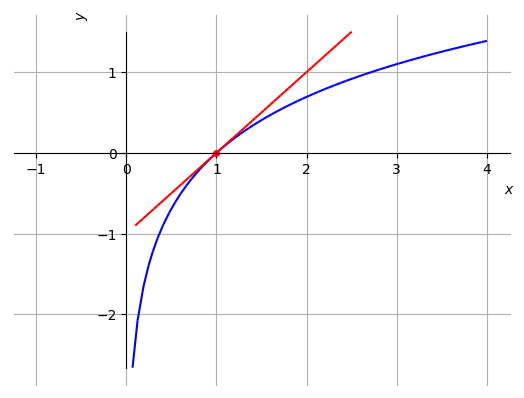
\includegraphics[width=0.7\textwidth]{fig_deriv/fig_deriv_exeresol_rt_ln}
    \caption{Esboço dos gráficos da função logarítmica natural e da reta tangente no ponto $x=1$.}
    \label{fig:deriv_exeresol_rt_ln}
  \end{figure}

  
  No \geogebra~ temos:
\begin{verbatim}
rt = derivada(log(x),1+log(1)
\end{verbatim}
\end{resol}

\begin{exeresol}
  Resolva a equação
  \begin{equation*}
    \frac{\dd}{\dd x}\arc\tg x = 1
  \end{equation*}
\end{exeresol}
\begin{resol}
  Lembrando que
  \begin{equation*}
    \frac{\dd}{\dd x}\arc\tg x = \frac{1}{1+x^2}
  \end{equation*}
  temos
  \begin{align*}
    \frac{\dd}{\dd x}\arc\tg x = 1 &\Rightarrow \frac{1}{1+x^2}=1\\
                                   &\Rightarrow 1+x^2 = 1 \\
                                   &\Rightarrow x^2 = 0 \\
                                   &\Rightarrow x = 0.
  \end{align*}
\end{resol}

\begin{exeresol}
  Calcule
  \begin{equation*}
    \frac{\dd}{\dd x}x^x
  \end{equation*}
\end{exeresol}
\begin{resol}
  Observamos que
  \begin{align*}
    y = x^x &\Rightarrow \ln y = \ln x^x \\
            &\Rightarrow \ln y = x\ln x. \\
  \end{align*}
  Agora, derivando em relação a $x$ ambos os lados desta equação, obtemos
  \begin{align*}
    \frac{\dd}{\dd x}\ln y = \frac{\dd}{\dd x}\left(x\ln x\right) &\Rightarrow \frac{1}{y}\frac{\dd y}{\dd x} = 1 + \ln x \\
                                                                  &\Rightarrow \frac{\dd y}{\dd x} = y(1 + \ln x) \\
                                                                  &\Rightarrow \frac{\dd x^x}{\dd x} = x^x(1 + \ln x).
  \end{align*}
\end{resol}

\subsection{Exercícios}

\begin{exer}
  Calcule a derivada em relação a $x$ das seguintes funções:
  \begin{enumerate}[a)]
  \item $f(x) = \log_2 x^2$
  \item $g(x) = \ln (xe^x)$
  \end{enumerate}
\end{exer}
\begin{resp}
  a)~$\displaystyle f'(x) = \frac{2}{x\ln 2}$; b)~$g'(x) = \frac{1+x}{x}$
\end{resp}

\begin{exer}
  Calcule a derivada em relação a $x$ das seguintes funções:
  \begin{enumerate}[a)]
  \item $f(x) = \sqrt[3]{x^2}$
  \item $g(x) = (1+2x)^e$
  \end{enumerate}
\end{exer}
\begin{resp}
  a)~$\displaystyle f'(x) = \frac{2}{3\sqrt[3]{x}}$; b)~$g'(x) = 2e(1+2x)^{e-1}$
\end{resp}

\begin{exer}
  Calcule
  \begin{equation*}
    \frac{\dd}{\dd x} (1+x)^x
  \end{equation*}
\end{exer}
\begin{resp}
  $x(1+x)^{x-1} + (1+x)^x\ln(1+x)$
\end{resp}

\begin{exer}
  Encontre a equação da reta tangente ao gráfico de $f(x) = \arc\tg x$ no ponto $x=0$.
\end{exer}
\begin{resp}
  $y=x$
\end{resp}

\section{Derivação implícita}\hypertarget{DerivImplicita}{}\label{sec:DerivImplicita}
Até o momento, trabalhamos apenas com funções descritas pela equação \(y=f(x)\). Esse tipo de função é chamada de \textbf{explícita}, pois \(y\) é expressa explicitamente em termos de \(x\). Porém, existem outras situações nas quais será necessário lidar com equações como

\[ y^2-x+1=0, \quad y^7-3y^5+7y^2-x\,{\rm cos}(x)=0\quad \mbox{ou}\quad y^2+x^4+15=0, \]

que definem uma relação \textbf{implícita} entre as variáveis \(x\) e \(y\). Em alguns casos, seremos capazes de expressar a variável \(y\) explicitamente em termos de \(x\). Por exemplo, dada a equação
 $$2y +x^2 y +1= x$$ não está na forma explícita $y = f (x )$ . Mesmo assim, esta equação ainda define $y$ como uma função  de $x$ , pois podemos escrevê-la como 
\matt{y=\frac{x-1}{x^2+2}} 
Caso quiséssemos calcular $y'$, poderíamos utilizar esta última expressão. 

Há equações em que  $x$ e $y$ podem definir mais do que uma função. Por exemplo $x^2+y^2=0$ que 
representa graficamente uma circunferência de centro $(0,0)$ e raio unitário (Figura \ref{fig:Circ00}). Explicitando a 
variável $y$ encontramos duas funções 
$$y=\pm\sqrt{1-x^2}$$

A função $y=+\sqrt{1-x^2}$ representa a semicircunferência superior (Figura \ref{fig:SemCirc1-1}) e $y=-\sqrt{1-x^2}$
representa a semicircunferência inferior (Figura \ref{fig:SemCirc-1+1}). 
\begin{figure}[H]
    \centering
    \subfigure[ $x^2+y^2=1$]{\label{fig:Circ00}%
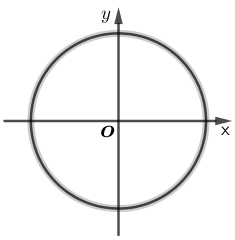
\includegraphics[width=3.5cm]{3-cap_derivadas/fig_deriv/CircunfDerivImplicita.png}}\hfill
\subfigure[$y=+\sqrt{1-x^2}$]{\label{fig:SemCirc1-1}%
\includegraphics[width=3.5cm]{3-cap_derivadas/fig_deriv/SemiCircsup.png}}\hfill
\subfigure[ $y=-\sqrt{1-x^2}$]{\label{fig:SemCirc-1+1}%
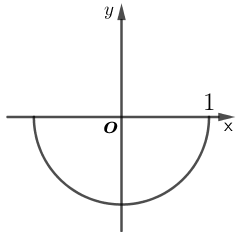
\includegraphics[width=3.5cm]{3-cap_derivadas/fig_deriv/SemiCircInf2}}
\caption{}\label{Circunf-x^2+y^2=1}
\end{figure}

Caso quiséssemos calcular $y'$ , poderíamos utilizar uma das expressões $y =\pm\sqrt{1-x^2}$. Ainda neste 
caso é possível explicitar a variável $y$, mesmo sabendo que parte do gráfico é suprimido neste 
processo. 

 Às vezes o processo para explicitar a variável $y$ é bastante longo e trabalhoso, como é o caso da 
expressão 
$$x^3+ y^3- 3xy=0$$
e até mesmo impossível por qualquer método elementar, como neste caso 
$$\sin(xy) - y = 0$$

O método da derivação implícita permitirá encontrar a derivada $y'$ sem a necessidade de explicitar 
a função como $y = f ( x)$. 

Para entender o método da derivação explícita, Considere, $y = y(x)$ definida implicitamente por
\begin{equation*}
  g(y(x)) = 0
\end{equation*}
A derivada $\dd y/\dd x$ pode ser calculada via regra da cadeia
\begin{equation*}
  \frac{\dd}{\dd x}g(y(x)) =0 \Rightarrow g'(y(x))\frac{\dd y}{\dd x} = 0
\end{equation*}

\begin{ex}
  Considere a equação da circunferência unitária
  \begin{equation*}
    x^2 + y^2 = 1
  \end{equation*}
  Para calcularmos $\dd y/\dd x$, fazemos
  \begin{align*}
    \frac{\dd}{\dd x}\left(x^2+y^2\right) = 0 &\Rightarrow 2x + \frac{\dd (2y)}{\dd y}\frac{\dd y}{\dd x}\\
                                                                &\Rightarrow 2x + 2y\frac{\dd y}{\dd x} = 0\\
                                                                &\Rightarrow \frac{\dd y}{\dd x} = -\frac{x}{y}
  \end{align*}
\end{ex}

\begin{exeresol}
  Usando derivação implícita, encontremos \(y'\) se:
  \begin{compactenum}[a)]
    \item \(y^2-x+1=0\)
    
    \begin{solution}
        \[ \begin{array}{rcl} \dfrac{d}{dx}\left[y^2-x+1\right]&=&\dfrac{d}{dx}[0]\\ 2yy'-1+ 0 &=& 0\\ 2yy' &=& 1. \end{array} \]
Logo,

\[ y' =\dfrac{1}{2y}. \]
    \end{solution}
    \item \(y^2+x^4-9=0\).
    
    \begin{solution}
        \[ \begin{array}{rcl} \dfrac{d}{dx}\left[y^2+x^4-9\right]&=&\dfrac{d}{dx}[0]\\ 2yy'+4x^3- 0 &=& 0\\ 2yy' &=& -4x^3 . \end{array} \]
Logo,

\[ y' =-\dfrac{2x^3}{y}. \]
    \end{solution}
    \item \(y^7-3y^5+7y^2-x{\rm cos}(x)=0\).
    
    \begin{solution}
        \[ \begin{array}{rcl} \dfrac{d}{dx}\left[y^7-3y^5+7y^2-x\,{\rm cos}(x)\right]&=&\dfrac{d}{dx}[0]\\ 7y^6y'-15y^4y'+14yy'-{\rm cos}(x)+x\,{\rm sen}(x) &=& 0\\ (7y^6-15y^4+14y)y' &=& {\rm cos}(x)-x\,{\rm sen}(x) . \end{array} \]
Logo,

\[ y' =\dfrac{{\rm cos}(x)-x\,{\rm sen}(x)}{7y^6-15y^4+14y}. \]
    \end{solution}
  \end{compactenum}
\end{exeresol}
\nota{No último exercício resolvido, as respostas apresentadas envolvem tanto \(x\) quanto \(y\). A fim de obter uma solução que envolva somente \(x\), teríamos de resolver a equação original, ou seja, obter \(y\) de forma explícita e, então substituir em cada uma das soluções dadas. Fazendo isto para os itens (a) e (b), temos que:

\[ {\rm (a)\quad} y^2-x+1=0\quad \Rightarrow \quad y=\pm \sqrt{x-1}\quad \Rightarrow \quad y' =\pm\dfrac{1}{2\sqrt{x-1}}. \] \[ {\rm (b)\quad} y^2+x^4-9=0\quad \Rightarrow \quad y=\pm \sqrt{9-x^4}\quad \Rightarrow \quad y' =\mp\dfrac{2x^3}{\sqrt{9-x^4}} \]
Porém, para o item (c) isto é impossível de ser feito, assim, somos forçados a deixar a fórmula de \(y'\) em termos de \(x\).}

\subsection{Exercícios}

\begin{exer}
 Determine a derivada $y'$ das curvas dadas implicitamente por: 
 \begin{multicols}{3}
 \begin{compactenum}[a)]
 \item $x^2+y^2=4$\item $xy^2+2y^3=x-2y$\item $x^2y^2+x\sin y=0$\item $e^{xy}=x+y-3$\item $y-\frac{x-y}{x+y}=0$\item $\tan y=xy-1$
 \end{compactenum}\end{multicols}
\end{exer}
\begin{exer}
Determine a equação da reta tangente e da reta normal ao gráfico de cada função abaixo, nos 
pontos indicados.
 \begin{compactenum}[a)]
 \item $\ln (xy)=x+y^2$ no ponto $P(-1,1)$. 
\item $x^3=y2^y$, no ponto em que a normal é vertical. 
\item $6x^2+ 13y^2= 19$ (elipse), nos pontos onde a normal é paralela à reta $26 x - 12y -7 = 0$. 
 \end{compactenum}
\end{exer}
\begin{exer}
Seja C a circunferência dada implicitamente por $x^2+y^2=1$ e $t$ a reta tangente à C no ponto de 
abscissa $x_0=\sqrt{2}/2$, como mostra a figura abaixo. Calcule o valor da área sombreada. 
\begin{figure}[H]
    \centering
    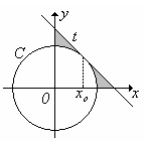
\includegraphics[scale=1.3]{3-cap_derivadas/fig_deriv/circsomb.png}
\end{figure}
\end{exer}
\begin{exer}
Determine a área do triângulo AOB na figura abaixo sabendo-se que $r$ é a reta tangente a curva C , 
dada implicitamente por e $e^{xy}+2\cos(x^2- 1)= 3x$, no ponto $A( 1, 0 ) $. 
\begin{figure}[H]
    \centering
    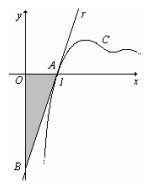
\includegraphics[scale=1.2]{3-cap_derivadas/fig_deriv/triangsomb.png}
   \end{figure}
\end{exer}
\section{Recapitulando}
Neste capítulo, apresentamos o conceito da \textbf{derivada}. Novamente, percebemos que esse conceito, assim como o de \textbf{continuidade}, depende da teoria de \textbf{limites}, e este limite é tão importante que possui a notação específica \(y'\). As definições da derivada e da \textbf{reta tangente} foram estabelecidas para um ponto dado. De certa forma, a derivada pode ser interpretada como a inclinação da reta tangente à curva \(y=f(x)\) em um ponto dado. Além disso, diferente do conceito de continuidade, podemos pensar na derivada como uma função.

Desde que a definição da derivada depende da obtenção de um limite, quando a variável se aproxima do ponto analisado, os conceitos de \hyperlink{DerivLaterais}{derivadas laterais} são estabelecidos. Além disso, a definição da reta normal à curva dada é apresentada. Depois disso, apresentamos as regras de derivação para as operações aritméticas, a derivada da composição de funções e o teorema da função inversa.

Tendo a teoria necessária para a obtenção da derivada, as derivadas de funções elementares foram apresentadas. Como a derivada de uma função é uma outra função, podemos recorrer repetidamente à obtenção da derivada destas novas funções, e a isto dá-se o nome \hyperlink{DerivOrdemSup}{derivadas de ordem superior}.


Por fim, apresentamos a \hyperlink{DerivImplicita} {derivação implícita}, teoria que lida com a obtenção da derivada de equações, na qual a função a ser derivada não necessariamente tem uma representação explícita. Exemplos foram desenvolvidos tentando ilustrar todos esses assuntos.

No próximo capítulo, apresentaremos algumas \textbf{aplicações da derivada}. Por exemplo, com ajuda da derivada de primeira e segunda ordem, aprenderemos métodos para analisar o comportamento de uma função em um conjunto dado e obteremos com uma maior precisão o seu gráfico.
\end{document}